\documentclass[twoside]{book}

% Packages required by doxygen
\usepackage{fixltx2e}
\usepackage{calc}
\usepackage{doxygen}
\usepackage[export]{adjustbox} % also loads graphicx
\usepackage{graphicx}
\usepackage[utf8]{inputenc}
\usepackage{makeidx}
\usepackage{multicol}
\usepackage{multirow}
\PassOptionsToPackage{warn}{textcomp}
\usepackage{textcomp}
\usepackage[nointegrals]{wasysym}
\usepackage[table]{xcolor}

% Font selection
\usepackage[T1]{fontenc}
\usepackage[scaled=.90]{helvet}
\usepackage{courier}
\usepackage{amssymb}
\usepackage{sectsty}
\renewcommand{\familydefault}{\sfdefault}
\allsectionsfont{%
  \fontseries{bc}\selectfont%
  \color{darkgray}%
}
\renewcommand{\DoxyLabelFont}{%
  \fontseries{bc}\selectfont%
  \color{darkgray}%
}
\newcommand{\+}{\discretionary{\mbox{\scriptsize$\hookleftarrow$}}{}{}}

% Page & text layout
\usepackage{geometry}
\geometry{%
  a4paper,%
  top=2.5cm,%
  bottom=2.5cm,%
  left=2.5cm,%
  right=2.5cm%
}
\tolerance=750
\hfuzz=15pt
\hbadness=750
\setlength{\emergencystretch}{15pt}
\setlength{\parindent}{0cm}
\setlength{\parskip}{3ex plus 2ex minus 2ex}
\makeatletter
\renewcommand{\paragraph}{%
  \@startsection{paragraph}{4}{0ex}{-1.0ex}{1.0ex}{%
    \normalfont\normalsize\bfseries\SS@parafont%
  }%
}
\renewcommand{\subparagraph}{%
  \@startsection{subparagraph}{5}{0ex}{-1.0ex}{1.0ex}{%
    \normalfont\normalsize\bfseries\SS@subparafont%
  }%
}
\makeatother

% Headers & footers
\usepackage{fancyhdr}
\pagestyle{fancyplain}
\fancyhead[LE]{\fancyplain{}{\bfseries\thepage}}
\fancyhead[CE]{\fancyplain{}{}}
\fancyhead[RE]{\fancyplain{}{\bfseries\leftmark}}
\fancyhead[LO]{\fancyplain{}{\bfseries\rightmark}}
\fancyhead[CO]{\fancyplain{}{}}
\fancyhead[RO]{\fancyplain{}{\bfseries\thepage}}
\fancyfoot[LE]{\fancyplain{}{}}
\fancyfoot[CE]{\fancyplain{}{}}
\fancyfoot[RE]{\fancyplain{}{\bfseries\scriptsize Generated by Doxygen }}
\fancyfoot[LO]{\fancyplain{}{\bfseries\scriptsize Generated by Doxygen }}
\fancyfoot[CO]{\fancyplain{}{}}
\fancyfoot[RO]{\fancyplain{}{}}
\renewcommand{\footrulewidth}{0.4pt}
\renewcommand{\chaptermark}[1]{%
  \markboth{#1}{}%
}
\renewcommand{\sectionmark}[1]{%
  \markright{\thesection\ #1}%
}

% Indices & bibliography
\usepackage{natbib}
\usepackage[titles]{tocloft}
\setcounter{tocdepth}{3}
\setcounter{secnumdepth}{5}
\makeindex

% Hyperlinks (required, but should be loaded last)
\usepackage{ifpdf}
\ifpdf
  \usepackage[pdftex,pagebackref=true]{hyperref}
\else
  \usepackage[ps2pdf,pagebackref=true]{hyperref}
\fi
\hypersetup{%
  colorlinks=true,%
  linkcolor=blue,%
  citecolor=blue,%
  unicode%
}

% Custom commands
\newcommand{\clearemptydoublepage}{%
  \newpage{\pagestyle{empty}\cleardoublepage}%
}

\usepackage{caption}
\captionsetup{labelsep=space,justification=centering,font={bf},singlelinecheck=off,skip=4pt,position=top}

%===== C O N T E N T S =====

\begin{document}

% Titlepage & ToC
\hypersetup{pageanchor=false,
             bookmarksnumbered=true,
             pdfencoding=unicode
            }
\pagenumbering{alph}
\begin{titlepage}
\vspace*{7cm}
\begin{center}%
{\Large software\+\_\+\+A\+P\+Is \\[1ex]\large 1.\+0.\+0 }\\
\vspace*{1cm}
{\large Generated by Doxygen 1.8.13}\\
\end{center}
\end{titlepage}
\clearemptydoublepage
\pagenumbering{roman}
\tableofcontents
\clearemptydoublepage
\pagenumbering{arabic}
\hypersetup{pageanchor=true}

%--- Begin generated contents ---
\chapter{Todo List}
\label{todo}
\Hypertarget{todo}

\begin{DoxyRefList}
\item[\label{todo__todo000001}%
\Hypertarget{todo__todo000001}%
Member \hyperlink{gpios_8h_a55f590722256813d85552b198b25440d}{set\+\_\+gpio} (long data)]verify this function 
\end{DoxyRefList}
\chapter{File Index}
\section{File List}
Here is a list of all documented files with brief descriptions\+:\begin{DoxyCompactList}
\item\contentsline{section}{/home/rady/caravel/caravel\+\_\+user\+\_\+project/caravel-\/sim-\/infrastructure/cocotb/interfaces/common\+\_\+functions/{\bfseries bitbang.\+h} }{\pageref{bitbang_8h}}{}
\item\contentsline{section}{/home/rady/caravel/caravel\+\_\+user\+\_\+project/caravel-\/sim-\/infrastructure/cocotb/interfaces/common\+\_\+functions/\hyperlink{common_8h}{common.\+h} }{\pageref{common_8h}}{}
\item\contentsline{section}{/home/rady/caravel/caravel\+\_\+user\+\_\+project/caravel-\/sim-\/infrastructure/cocotb/interfaces/common\+\_\+functions/\hyperlink{gpios_8h}{gpios.\+h} }{\pageref{gpios_8h}}{}
\item\contentsline{section}{/home/rady/caravel/caravel\+\_\+user\+\_\+project/caravel-\/sim-\/infrastructure/cocotb/interfaces/common\+\_\+functions/\hyperlink{irq__api_8h}{irq\+\_\+api.\+h} }{\pageref{irq__api_8h}}{}
\item\contentsline{section}{/home/rady/caravel/caravel\+\_\+user\+\_\+project/caravel-\/sim-\/infrastructure/cocotb/interfaces/common\+\_\+functions/\hyperlink{la_8h}{la.\+h} }{\pageref{la_8h}}{}
\item\contentsline{section}{/home/rady/caravel/caravel\+\_\+user\+\_\+project/caravel-\/sim-\/infrastructure/cocotb/interfaces/common\+\_\+functions/\hyperlink{mgmt__gpio_8h}{mgmt\+\_\+gpio.\+h} }{\pageref{mgmt__gpio_8h}}{}
\item\contentsline{section}{/home/rady/caravel/caravel\+\_\+user\+\_\+project/caravel-\/sim-\/infrastructure/cocotb/interfaces/common\+\_\+functions/\hyperlink{spi__master_8h}{spi\+\_\+master.\+h} }{\pageref{spi__master_8h}}{}
\item\contentsline{section}{/home/rady/caravel/caravel\+\_\+user\+\_\+project/caravel-\/sim-\/infrastructure/cocotb/interfaces/common\+\_\+functions/\hyperlink{timer0_8h}{timer0.\+h} }{\pageref{timer0_8h}}{}
\item\contentsline{section}{/home/rady/caravel/caravel\+\_\+user\+\_\+project/caravel-\/sim-\/infrastructure/cocotb/interfaces/common\+\_\+functions/\hyperlink{uart__api_8h}{uart\+\_\+api.\+h} }{\pageref{uart__api_8h}}{}
\item\contentsline{section}{/home/rady/caravel/caravel\+\_\+user\+\_\+project/caravel-\/sim-\/infrastructure/cocotb/interfaces/common\+\_\+functions/\hyperlink{user__addr__space_8h}{user\+\_\+addr\+\_\+space.\+h} }{\pageref{user__addr__space_8h}}{}
\end{DoxyCompactList}

\chapter{File Documentation}
\hypertarget{common_8h}{}\section{/home/rady/caravel/caravel\+\_\+user\+\_\+project/caravel-\/dynamic-\/sims/cocotb/interfaces/common\+\_\+functions/common.h File Reference}
\label{common_8h}\index{/home/rady/caravel/caravel\+\_\+user\+\_\+project/caravel-\/dynamic-\/sims/cocotb/interfaces/common\+\_\+functions/common.\+h@{/home/rady/caravel/caravel\+\_\+user\+\_\+project/caravel-\/dynamic-\/sims/cocotb/interfaces/common\+\_\+functions/common.\+h}}
{\ttfamily \#include $<$defs.\+h$>$}\newline
{\ttfamily \#include $<$stub.\+c$>$}\newline
{\ttfamily \#include $<$uart.\+h$>$}\newline
{\ttfamily \#include $<$irq\+\_\+vex.\+h$>$}\newline
{\ttfamily \#include $<$gpios.\+h$>$}\newline
{\ttfamily \#include $<$timer0.\+h$>$}\newline
{\ttfamily \#include $<$mgmt\+\_\+gpio.\+h$>$}\newline
{\ttfamily \#include $<$irq\+\_\+api.\+h$>$}\newline
{\ttfamily \#include $<$la.\+h$>$}\newline
{\ttfamily \#include $<$uart\+\_\+api.\+h$>$}\newline
{\ttfamily \#include $<$spi\+\_\+master.\+h$>$}\newline
{\ttfamily \#include $<$user\+\_\+addr\+\_\+space.\+h$>$}\newline
Include dependency graph for common.\+h\+:\nopagebreak
\begin{figure}[H]
\begin{center}
\leavevmode
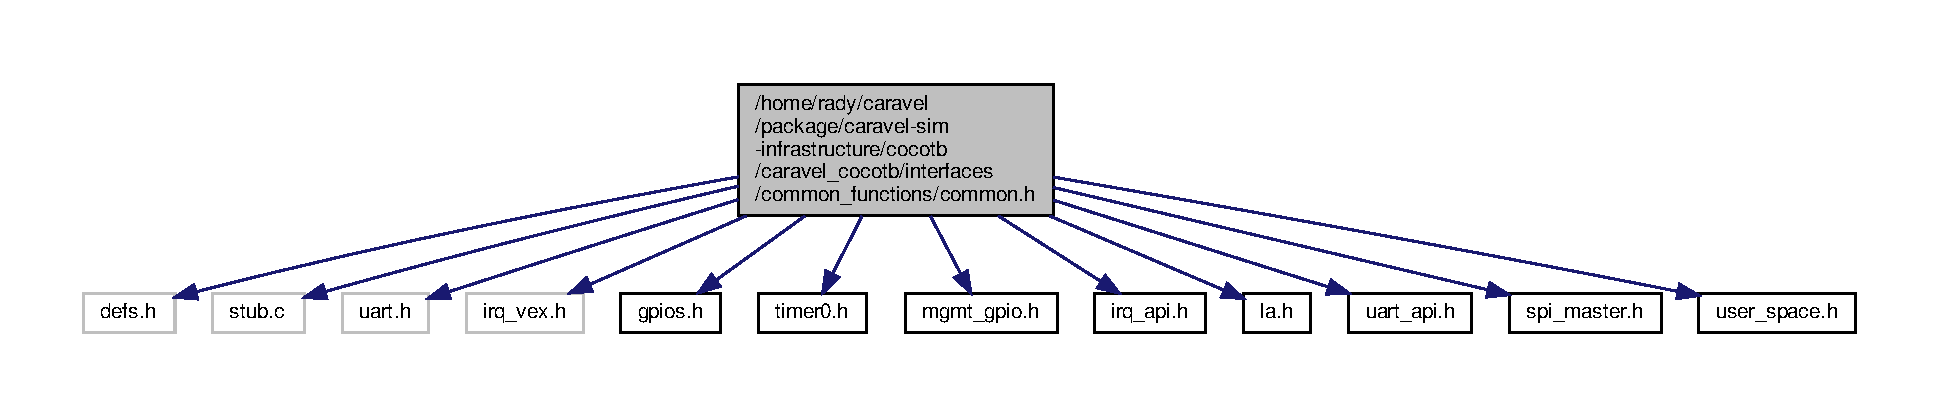
\includegraphics[width=350pt]{common_8h__incl}
\end{center}
\end{figure}
\subsection*{Functions}
\begin{DoxyCompactItemize}
\item 
void \hyperlink{common_8h_af79fbe355fd538621db12e3ae9e3e6b8}{enable\+\_\+user\+\_\+interface} ()
\item 
void \hyperlink{common_8h_a37a92e81df76732622207204976178f9}{enable\+\_\+hk\+\_\+spi} (bool is\+\_\+enable)
\item 
void \hyperlink{common_8h_a875e99bdc81b2f0c925af03d4881438c}{dummy\+\_\+delay} (int num)
\end{DoxyCompactItemize}


\subsection{Function Documentation}
\mbox{\Hypertarget{common_8h_a875e99bdc81b2f0c925af03d4881438c}\label{common_8h_a875e99bdc81b2f0c925af03d4881438c}} 
\index{common.\+h@{common.\+h}!dummy\+\_\+delay@{dummy\+\_\+delay}}
\index{dummy\+\_\+delay@{dummy\+\_\+delay}!common.\+h@{common.\+h}}
\subsubsection{\texorpdfstring{dummy\+\_\+delay()}{dummy\_delay()}}
{\footnotesize\ttfamily void dummy\+\_\+delay (\begin{DoxyParamCaption}\item[{int}]{num }\end{DoxyParamCaption})}

Insert delay


\begin{DoxyParams}{Parameters}
{\em num} & number of delays steps. step is increment local variable and check it\textquotesingle{}s value \\
\hline
\end{DoxyParams}
\mbox{\Hypertarget{common_8h_a37a92e81df76732622207204976178f9}\label{common_8h_a37a92e81df76732622207204976178f9}} 
\index{common.\+h@{common.\+h}!enable\+\_\+hk\+\_\+spi@{enable\+\_\+hk\+\_\+spi}}
\index{enable\+\_\+hk\+\_\+spi@{enable\+\_\+hk\+\_\+spi}!common.\+h@{common.\+h}}
\subsubsection{\texorpdfstring{enable\+\_\+hk\+\_\+spi()}{enable\_hk\_spi()}}
{\footnotesize\ttfamily void enable\+\_\+hk\+\_\+spi (\begin{DoxyParamCaption}\item[{bool}]{is\+\_\+enable }\end{DoxyParamCaption})}

Enable or disable the housekeeping S\+PI This function writes to the housekeeping disenable register inside the housekeeping \begin{DoxyNote}{Note}
When this register asserted housekeeping S\+PI can\textquotesingle{}t be used and G\+P\+I\+Os\mbox{[}3\mbox{]} which is C\+SB can be used as any other Caravel G\+P\+I\+Os
\end{DoxyNote}
\begin{DoxyWarning}{Warning}
By default the housekeeping S\+PI is enabled to use G\+P\+I\+Os\mbox{[}3\mbox{]} freely it should be disabled.
\end{DoxyWarning}

\begin{DoxyParams}{Parameters}
{\em is\+\_\+enable} & when 1 (true) housekeeping is active, 0 (false) housekeeping is disabled \\
\hline
\end{DoxyParams}
\mbox{\Hypertarget{common_8h_af79fbe355fd538621db12e3ae9e3e6b8}\label{common_8h_af79fbe355fd538621db12e3ae9e3e6b8}} 
\index{common.\+h@{common.\+h}!enable\+\_\+user\+\_\+interface@{enable\+\_\+user\+\_\+interface}}
\index{enable\+\_\+user\+\_\+interface@{enable\+\_\+user\+\_\+interface}!common.\+h@{common.\+h}}
\subsubsection{\texorpdfstring{enable\+\_\+user\+\_\+interface()}{enable\_user\_interface()}}
{\footnotesize\ttfamily void enable\+\_\+user\+\_\+interface (\begin{DoxyParamCaption}{ }\end{DoxyParamCaption})}

Enable communication between firmware and user project \begin{DoxyWarning}{Warning}
This necessary when reading or writing are needed between wishbone and user project if interface isn\textquotesingle{}t enabled no ack would be receive and the writing or reading command will be stuck 
\end{DoxyWarning}

\hypertarget{gpios_8h}{}\section{/home/rady/caravel/caravel\+\_\+user\+\_\+project/caravel-\/sim-\/infrastructure/cocotb/interfaces/common\+\_\+functions/gpios.h File Reference}
\label{gpios_8h}\index{/home/rady/caravel/caravel\+\_\+user\+\_\+project/caravel-\/sim-\/infrastructure/cocotb/interfaces/common\+\_\+functions/gpios.\+h@{/home/rady/caravel/caravel\+\_\+user\+\_\+project/caravel-\/sim-\/infrastructure/cocotb/interfaces/common\+\_\+functions/gpios.\+h}}
This graph shows which files directly or indirectly include this file\+:
\nopagebreak
\begin{figure}[H]
\begin{center}
\leavevmode
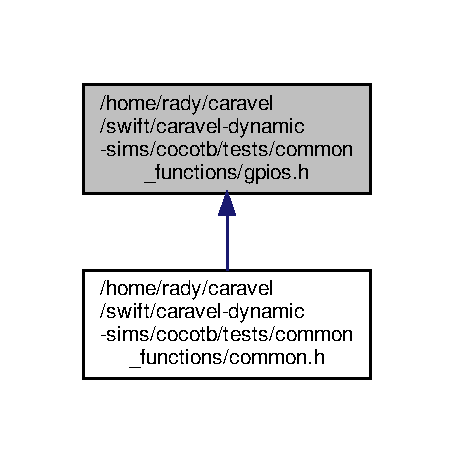
\includegraphics[width=215pt]{gpios_8h__dep__incl}
\end{center}
\end{figure}
\subsection*{Enumerations}
\begin{DoxyCompactItemize}
\item 
enum \hyperlink{gpios_8h_a620d533a2ccc5296d2f6c8b95bf89fe1}{gpio\+\_\+mode} 
\end{DoxyCompactItemize}
\subsection*{Functions}
\begin{DoxyCompactItemize}
\item 
void \hyperlink{gpios_8h_a855aacde2c3eb9f09f7ca6d4ee44b57a}{configure\+\_\+all\+\_\+gpios} (enum \hyperlink{gpios_8h_a620d533a2ccc5296d2f6c8b95bf89fe1}{gpio\+\_\+mode} config)
\item 
void \hyperlink{gpios_8h_a7d48a49426f2c9c379660611de769c29}{gpio\+\_\+config\+\_\+load} ()
\item 
void \hyperlink{gpios_8h_a60b4f4fbfae8495880881b1d4da68725}{configure\+\_\+gpio} (int gpio\+\_\+num, enum \hyperlink{gpios_8h_a620d533a2ccc5296d2f6c8b95bf89fe1}{gpio\+\_\+mode} config)
\item 
void \hyperlink{gpios_8h_a381a8a44c3dad81f0a46e202533dba8a}{set\+\_\+gpio\+\_\+l} (unsigned int data)
\item 
void \hyperlink{gpios_8h_ac6950e132b8bd925bb1ede3d18631f05}{set\+\_\+gpio\+\_\+h} (unsigned int data)
\item 
void \hyperlink{gpios_8h_a55f590722256813d85552b198b25440d}{set\+\_\+gpio} (long data)
\item 
unsigned int \hyperlink{gpios_8h_a48dd1cdca7124e34b86b729d7355ce04}{get\+\_\+gpio\+\_\+h} ()
\item 
unsigned int \hyperlink{gpios_8h_a5b3a80032bca3d58fb29a598b8524fb1}{get\+\_\+gpio\+\_\+l} ()
\item 
void \hyperlink{gpios_8h_ae04c0971756bf7f833129bf0b6f6d547}{wait\+\_\+gpio\+\_\+l} (unsigned int data)
\item 
void \hyperlink{gpios_8h_a9fb980ee2469d57c9d37eed263f1864d}{wait\+\_\+gpio\+\_\+h} (unsigned int data)
\item 
void \hyperlink{gpios_8h_a4f971ec71379f092d9b616ec6e40bde1}{wait\+\_\+gpio\+\_\+l\+\_\+masked} (unsigned int data, unsigned int mask)
\item 
void \hyperlink{gpios_8h_ad071916d2d8c21af15b9dd1ed385b437}{wait\+\_\+gpio\+\_\+h\+\_\+masked} (unsigned int data, unsigned int mask)
\end{DoxyCompactItemize}


\subsection{Enumeration Type Documentation}
\mbox{\Hypertarget{gpios_8h_a620d533a2ccc5296d2f6c8b95bf89fe1}\label{gpios_8h_a620d533a2ccc5296d2f6c8b95bf89fe1}} 
\index{gpios.\+h@{gpios.\+h}!gpio\+\_\+mode@{gpio\+\_\+mode}}
\index{gpio\+\_\+mode@{gpio\+\_\+mode}!gpios.\+h@{gpios.\+h}}
\subsubsection{\texorpdfstring{gpio\+\_\+mode}{gpio\_mode}}
{\footnotesize\ttfamily enum \hyperlink{gpios_8h_a620d533a2ccc5296d2f6c8b95bf89fe1}{gpio\+\_\+mode}}

G\+P\+I\+Os possible modes \hypertarget{user__addr__space_8h_multi_row}{}
\tabulinesep=1mm
\begin{longtabu} spread 0pt [c]{*{2}{|X[-1]}|}
\caption{Enumerator gpio\+\_\+mode}\label{user__addr__space_8h_multi_row}\\
\hline
\rowcolor{\tableheadbgcolor}\textbf{ name}&\textbf{ description }\\\cline{1-2}
\endfirsthead
\hline
\endfoot
\hline
\rowcolor{\tableheadbgcolor}\textbf{ name}&\textbf{ description }\\\cline{1-2}
\endhead
G\+P\+I\+O\+\_\+\+M\+O\+D\+E\+\_\+\+M\+G\+M\+T\+\_\+\+S\+T\+D\+\_\+\+I\+N\+P\+U\+T\+\_\+\+N\+O\+P\+U\+LL&Management input with no pull (floating is read as Z) \\\cline{1-2}
G\+P\+I\+O\+\_\+\+M\+O\+D\+E\+\_\+\+M\+G\+M\+T\+\_\+\+S\+T\+D\+\_\+\+I\+N\+P\+U\+T\+\_\+\+P\+U\+L\+L\+D\+O\+WN&Management input pull-\/down (floating is read as 0) \\\cline{1-2}
G\+P\+I\+O\+\_\+\+M\+O\+D\+E\+\_\+\+M\+G\+M\+T\+\_\+\+S\+T\+D\+\_\+\+I\+N\+P\+U\+T\+\_\+\+P\+U\+L\+L\+UP&Management input pull-\/up (floating is read as 1) \\\cline{1-2}
G\+P\+I\+O\+\_\+\+M\+O\+D\+E\+\_\+\+M\+G\+M\+T\+\_\+\+S\+T\+D\+\_\+\+O\+U\+T\+P\+UT&Management output \\\cline{1-2}
G\+P\+I\+O\+\_\+\+M\+O\+D\+E\+\_\+\+M\+G\+M\+T\+\_\+\+S\+T\+D\+\_\+\+B\+I\+D\+I\+R\+E\+C\+T\+I\+O\+N\+AL&Management bi-\/direction \\\cline{1-2}
G\+P\+I\+O\+\_\+\+M\+O\+D\+E\+\_\+\+M\+G\+M\+T\+\_\+\+S\+T\+D\+\_\+\+A\+N\+A\+L\+OG&Management Analog \\\cline{1-2}
G\+P\+I\+O\+\_\+\+M\+O\+D\+E\+\_\+\+U\+S\+E\+R\+\_\+\+S\+T\+D\+\_\+\+I\+N\+P\+U\+T\+\_\+\+N\+O\+P\+U\+LL&User input with no pull (floating is read as Z) \\\cline{1-2}
G\+P\+I\+O\+\_\+\+M\+O\+D\+E\+\_\+\+U\+S\+E\+R\+\_\+\+S\+T\+D\+\_\+\+I\+N\+P\+U\+T\+\_\+\+P\+U\+L\+L\+D\+O\+WN&User input pull-\/down (floating is read as 0) \\\cline{1-2}
G\+P\+I\+O\+\_\+\+M\+O\+D\+E\+\_\+\+U\+S\+E\+R\+\_\+\+S\+T\+D\+\_\+\+I\+N\+P\+U\+T\+\_\+\+P\+U\+L\+L\+UP&User input pull-\/up (floating is read as 1) \\\cline{1-2}
G\+P\+I\+O\+\_\+\+M\+O\+D\+E\+\_\+\+U\+S\+E\+R\+\_\+\+S\+T\+D\+\_\+\+O\+U\+T\+P\+UT&User output \\\cline{1-2}
G\+P\+I\+O\+\_\+\+M\+O\+D\+E\+\_\+\+U\+S\+E\+R\+\_\+\+S\+T\+D\+\_\+\+B\+I\+D\+I\+R\+E\+C\+T\+I\+O\+N\+AL&User bi-\/direction \\\cline{1-2}
G\+P\+I\+O\+\_\+\+M\+O\+D\+E\+\_\+\+U\+S\+E\+R\+\_\+\+S\+T\+D\+\_\+\+O\+U\+T\+\_\+\+M\+O\+N\+I\+T\+O\+R\+ED&User Monitor same as output \\\cline{1-2}
G\+P\+I\+O\+\_\+\+M\+O\+D\+E\+\_\+\+U\+S\+E\+R\+\_\+\+S\+T\+D\+\_\+\+A\+N\+A\+L\+OG&User Analog \\\cline{1-2}
\end{longtabu}


\subsection{Function Documentation}
\mbox{\Hypertarget{gpios_8h_a855aacde2c3eb9f09f7ca6d4ee44b57a}\label{gpios_8h_a855aacde2c3eb9f09f7ca6d4ee44b57a}} 
\index{gpios.\+h@{gpios.\+h}!configure\+\_\+all\+\_\+gpios@{configure\+\_\+all\+\_\+gpios}}
\index{configure\+\_\+all\+\_\+gpios@{configure\+\_\+all\+\_\+gpios}!gpios.\+h@{gpios.\+h}}
\subsubsection{\texorpdfstring{configure\+\_\+all\+\_\+gpios()}{configure\_all\_gpios()}}
{\footnotesize\ttfamily void configure\+\_\+all\+\_\+gpios (\begin{DoxyParamCaption}\item[{enum \hyperlink{gpios_8h_a620d533a2ccc5296d2f6c8b95bf89fe1}{gpio\+\_\+mode}}]{config }\end{DoxyParamCaption})}

Configure all G\+P\+I\+Os with the config


\begin{DoxyParams}{Parameters}
{\em config} & is configuration of type gpio\+\_\+mode\\
\hline
\end{DoxyParams}
\begin{DoxyNote}{Note}
These configurations will not be change the G\+P\+I\+Os modes until calling \hyperlink{gpios_8h_a7d48a49426f2c9c379660611de769c29}{gpio\+\_\+config\+\_\+load()} 
\end{DoxyNote}
\mbox{\Hypertarget{gpios_8h_a60b4f4fbfae8495880881b1d4da68725}\label{gpios_8h_a60b4f4fbfae8495880881b1d4da68725}} 
\index{gpios.\+h@{gpios.\+h}!configure\+\_\+gpio@{configure\+\_\+gpio}}
\index{configure\+\_\+gpio@{configure\+\_\+gpio}!gpios.\+h@{gpios.\+h}}
\subsubsection{\texorpdfstring{configure\+\_\+gpio()}{configure\_gpio()}}
{\footnotesize\ttfamily void configure\+\_\+gpio (\begin{DoxyParamCaption}\item[{int}]{gpio\+\_\+num,  }\item[{enum \hyperlink{gpios_8h_a620d533a2ccc5296d2f6c8b95bf89fe1}{gpio\+\_\+mode}}]{config }\end{DoxyParamCaption})}

Configure one G\+P\+IO with the input config


\begin{DoxyParams}{Parameters}
{\em config} & is configuration of type gpio\+\_\+mode \\
\hline
{\em gpio\+\_\+num} & is G\+P\+IO number it can have values from 0 to 37\\
\hline
\end{DoxyParams}
\begin{DoxyNote}{Note}
These configurations will not be change the G\+P\+I\+Os modes until calling \hyperlink{gpios_8h_a7d48a49426f2c9c379660611de769c29}{gpio\+\_\+config\+\_\+load()} 
\end{DoxyNote}
\mbox{\Hypertarget{gpios_8h_a48dd1cdca7124e34b86b729d7355ce04}\label{gpios_8h_a48dd1cdca7124e34b86b729d7355ce04}} 
\index{gpios.\+h@{gpios.\+h}!get\+\_\+gpio\+\_\+h@{get\+\_\+gpio\+\_\+h}}
\index{get\+\_\+gpio\+\_\+h@{get\+\_\+gpio\+\_\+h}!gpios.\+h@{gpios.\+h}}
\subsubsection{\texorpdfstring{get\+\_\+gpio\+\_\+h()}{get\_gpio\_h()}}
{\footnotesize\ttfamily unsigned int get\+\_\+gpio\+\_\+h (\begin{DoxyParamCaption}{ }\end{DoxyParamCaption})}

Read the highest 6 G\+P\+I\+Os G\+P\+I\+OS\mbox{[}37\+:32\mbox{]} \begin{DoxyNote}{Note}
For Reading value from the G\+P\+I\+Os, the G\+P\+IO should be configured as management input. otherwise 0 would be read 
\end{DoxyNote}
\mbox{\Hypertarget{gpios_8h_a5b3a80032bca3d58fb29a598b8524fb1}\label{gpios_8h_a5b3a80032bca3d58fb29a598b8524fb1}} 
\index{gpios.\+h@{gpios.\+h}!get\+\_\+gpio\+\_\+l@{get\+\_\+gpio\+\_\+l}}
\index{get\+\_\+gpio\+\_\+l@{get\+\_\+gpio\+\_\+l}!gpios.\+h@{gpios.\+h}}
\subsubsection{\texorpdfstring{get\+\_\+gpio\+\_\+l()}{get\_gpio\_l()}}
{\footnotesize\ttfamily unsigned int get\+\_\+gpio\+\_\+l (\begin{DoxyParamCaption}{ }\end{DoxyParamCaption})}

Read low 32 G\+P\+I\+Os G\+P\+I\+OS\mbox{[}31\+:0\mbox{]} \begin{DoxyNote}{Note}
For Reading value from the G\+P\+I\+Os, the G\+P\+IO should be configured as management input. otherwise 0 would be read 
\end{DoxyNote}
\mbox{\Hypertarget{gpios_8h_a7d48a49426f2c9c379660611de769c29}\label{gpios_8h_a7d48a49426f2c9c379660611de769c29}} 
\index{gpios.\+h@{gpios.\+h}!gpio\+\_\+config\+\_\+load@{gpio\+\_\+config\+\_\+load}}
\index{gpio\+\_\+config\+\_\+load@{gpio\+\_\+config\+\_\+load}!gpios.\+h@{gpios.\+h}}
\subsubsection{\texorpdfstring{gpio\+\_\+config\+\_\+load()}{gpio\_config\_load()}}
{\footnotesize\ttfamily void gpio\+\_\+config\+\_\+load (\begin{DoxyParamCaption}{ }\end{DoxyParamCaption})}

Load the configurations changes to the G\+P\+I\+Os \mbox{\Hypertarget{gpios_8h_a55f590722256813d85552b198b25440d}\label{gpios_8h_a55f590722256813d85552b198b25440d}} 
\index{gpios.\+h@{gpios.\+h}!set\+\_\+gpio@{set\+\_\+gpio}}
\index{set\+\_\+gpio@{set\+\_\+gpio}!gpios.\+h@{gpios.\+h}}
\subsubsection{\texorpdfstring{set\+\_\+gpio()}{set\_gpio()}}
{\footnotesize\ttfamily void set\+\_\+gpio (\begin{DoxyParamCaption}\item[{long}]{data }\end{DoxyParamCaption})}

Write to the 38 G\+P\+I\+Os G\+P\+I\+OS\mbox{[}37\+:0\mbox{]} \begin{DoxyNote}{Note}
For writing by this function to be seen at the G\+P\+IO the G\+P\+IO has to be configured as management output
\end{DoxyNote}

\begin{DoxyParams}{Parameters}
{\em data} & is the data sent to the G\+P\+I\+Os\\
\hline
\end{DoxyParams}
Examples\+: \begin{DoxyItemize}
\item 
\begin{DoxyCode}
\hyperlink{gpios_8h_a55f590722256813d85552b198b25440d}{set\_gpio}(0x1); \textcolor{comment}{// write 1 to GPIO [0] and write 0 in the remaining 37 GPIOs }
\end{DoxyCode}
 \item 
\begin{DoxyCode}
\hyperlink{gpios_8h_a55f590722256813d85552b198b25440d}{set\_gpio}(0x5); \textcolor{comment}{// write 1 to GPIO [0] and GPIO [3] and write 0 in the remaining 36 GPIOs}
\end{DoxyCode}
 \item 
\begin{DoxyCode}
\hyperlink{gpios_8h_a55f590722256813d85552b198b25440d}{set\_gpio}(0x100000000); \textcolor{comment}{// write 1 to GPIO [32] and write 0 in the remaining 36 GPIOs}
\end{DoxyCode}
\end{DoxyItemize}
\begin{DoxyRefDesc}{Todo}
\item[\hyperlink{todo__todo000001}{Todo}]verify this function \end{DoxyRefDesc}
\mbox{\Hypertarget{gpios_8h_ac6950e132b8bd925bb1ede3d18631f05}\label{gpios_8h_ac6950e132b8bd925bb1ede3d18631f05}} 
\index{gpios.\+h@{gpios.\+h}!set\+\_\+gpio\+\_\+h@{set\+\_\+gpio\+\_\+h}}
\index{set\+\_\+gpio\+\_\+h@{set\+\_\+gpio\+\_\+h}!gpios.\+h@{gpios.\+h}}
\subsubsection{\texorpdfstring{set\+\_\+gpio\+\_\+h()}{set\_gpio\_h()}}
{\footnotesize\ttfamily void set\+\_\+gpio\+\_\+h (\begin{DoxyParamCaption}\item[{unsigned int}]{data }\end{DoxyParamCaption})}

Write to the highest 6 G\+P\+I\+Os G\+P\+I\+OS\mbox{[}37\+:32\mbox{]} \begin{DoxyNote}{Note}
For writing by this function to be seen at the G\+P\+IO the G\+P\+IO has to be configured as management output
\end{DoxyNote}

\begin{DoxyParams}{Parameters}
{\em data} & is the data sent to the G\+P\+I\+Os\\
\hline
\end{DoxyParams}
Examples\+: \begin{DoxyItemize}
\item 
\begin{DoxyCode}
\hyperlink{gpios_8h_ac6950e132b8bd925bb1ede3d18631f05}{set\_gpio\_h}(0x1); \textcolor{comment}{// write 1 to GPIO [32] and write 0 in the remaining 5 GPIOs}
\end{DoxyCode}
 \item 
\begin{DoxyCode}
\hyperlink{gpios_8h_ac6950e132b8bd925bb1ede3d18631f05}{set\_gpio\_h}(0x5); \textcolor{comment}{// write 1 to GPIO [32] and 34 and write 0 in the remaining 4 GPIOs}
\end{DoxyCode}
 \end{DoxyItemize}
\mbox{\Hypertarget{gpios_8h_a381a8a44c3dad81f0a46e202533dba8a}\label{gpios_8h_a381a8a44c3dad81f0a46e202533dba8a}} 
\index{gpios.\+h@{gpios.\+h}!set\+\_\+gpio\+\_\+l@{set\+\_\+gpio\+\_\+l}}
\index{set\+\_\+gpio\+\_\+l@{set\+\_\+gpio\+\_\+l}!gpios.\+h@{gpios.\+h}}
\subsubsection{\texorpdfstring{set\+\_\+gpio\+\_\+l()}{set\_gpio\_l()}}
{\footnotesize\ttfamily void set\+\_\+gpio\+\_\+l (\begin{DoxyParamCaption}\item[{unsigned int}]{data }\end{DoxyParamCaption})}

Write to the low 32 G\+P\+I\+Os G\+P\+I\+OS\mbox{[}31\+:0\mbox{]} \begin{DoxyNote}{Note}
For writing by this function to be seen at the G\+P\+IO the G\+P\+IO has to be configured as management output
\end{DoxyNote}

\begin{DoxyParams}{Parameters}
{\em data} & is the data sent to the G\+P\+I\+Os\\
\hline
\end{DoxyParams}
Examples\+: \begin{DoxyItemize}
\item 
\begin{DoxyCode}
\hyperlink{gpios_8h_a381a8a44c3dad81f0a46e202533dba8a}{set\_gpio\_l}(0x1); \textcolor{comment}{// write 1 to GPIO [0] and write 0 in the remaining 31 GPIOs }
\end{DoxyCode}
 \item 
\begin{DoxyCode}
\hyperlink{gpios_8h_a381a8a44c3dad81f0a46e202533dba8a}{set\_gpio\_l}(0x5); \textcolor{comment}{// write 1 to GPIO [0] and GPIO [3] and write 0 in the remaining 30 GPIOs}
\end{DoxyCode}
 \end{DoxyItemize}
\mbox{\Hypertarget{gpios_8h_a9fb980ee2469d57c9d37eed263f1864d}\label{gpios_8h_a9fb980ee2469d57c9d37eed263f1864d}} 
\index{gpios.\+h@{gpios.\+h}!wait\+\_\+gpio\+\_\+h@{wait\+\_\+gpio\+\_\+h}}
\index{wait\+\_\+gpio\+\_\+h@{wait\+\_\+gpio\+\_\+h}!gpios.\+h@{gpios.\+h}}
\subsubsection{\texorpdfstring{wait\+\_\+gpio\+\_\+h()}{wait\_gpio\_h()}}
{\footnotesize\ttfamily void wait\+\_\+gpio\+\_\+h (\begin{DoxyParamCaption}\item[{unsigned int}]{data }\end{DoxyParamCaption})}

wait over the highest 6 G\+P\+I\+Os to equal the data passed \begin{DoxyNote}{Note}
For writing by this function to be seen at the G\+P\+IO the G\+P\+IO has to be configured as management output
\end{DoxyNote}

\begin{DoxyParams}{Parameters}
{\em data} & is the data that should wait until sent to the G\+P\+I\+Os\\
\hline
\end{DoxyParams}
Examples\+: \begin{DoxyItemize}
\item 
\begin{DoxyCode}
\hyperlink{gpios_8h_a9fb980ee2469d57c9d37eed263f1864d}{wait\_gpio\_h}(0x1); \textcolor{comment}{// function would return only when GPIO [32]==1 and rest of 5 GPIOs = 0  }
\end{DoxyCode}
 \item 
\begin{DoxyCode}
\hyperlink{gpios_8h_a9fb980ee2469d57c9d37eed263f1864d}{wait\_gpio\_h}(0x5); \textcolor{comment}{// function would return only when GPIO [32]==1 and GPIO [34]==1 and rest of 4
       GPIOs = 0 }
\end{DoxyCode}
 \end{DoxyItemize}
\mbox{\Hypertarget{gpios_8h_ad071916d2d8c21af15b9dd1ed385b437}\label{gpios_8h_ad071916d2d8c21af15b9dd1ed385b437}} 
\index{gpios.\+h@{gpios.\+h}!wait\+\_\+gpio\+\_\+h\+\_\+masked@{wait\+\_\+gpio\+\_\+h\+\_\+masked}}
\index{wait\+\_\+gpio\+\_\+h\+\_\+masked@{wait\+\_\+gpio\+\_\+h\+\_\+masked}!gpios.\+h@{gpios.\+h}}
\subsubsection{\texorpdfstring{wait\+\_\+gpio\+\_\+h\+\_\+masked()}{wait\_gpio\_h\_masked()}}
{\footnotesize\ttfamily void wait\+\_\+gpio\+\_\+h\+\_\+masked (\begin{DoxyParamCaption}\item[{unsigned int}]{data,  }\item[{unsigned int}]{mask }\end{DoxyParamCaption})}

wait over the masked highest 6 G\+P\+I\+Os to equal the data passed \begin{DoxyNote}{Note}
For writing by this function to be seen at the G\+P\+IO the G\+P\+IO has to be configured as management output
\end{DoxyNote}

\begin{DoxyParams}{Parameters}
{\em data} & is the data that should wait until sent to the G\+P\+I\+Os \\
\hline
{\em mask} & mask over the each G\+P\+IO if the mask value is 0 the this G\+P\+IO value are ignored\\
\hline
\end{DoxyParams}
Examples\+: \begin{DoxyItemize}
\item 
\begin{DoxyCode}
\hyperlink{gpios_8h_ad071916d2d8c21af15b9dd1ed385b437}{wait\_gpio\_h\_masked}(0x1,0xF); \textcolor{comment}{// function would return only when GPIO [32]==1 and GPIO
       [35:33]==0 and don't care about the rest of GPIOs  }
\end{DoxyCode}
 \item 
\begin{DoxyCode}
\hyperlink{gpios_8h_ad071916d2d8c21af15b9dd1ed385b437}{wait\_gpio\_h\_masked}(0x5,0x7); \textcolor{comment}{// function would return only when GPIO [32]==1 and GPIO
       [34]==1 and GPIO [33]==0 and don't care about the rest of GPIOs }
\end{DoxyCode}
 \end{DoxyItemize}
\mbox{\Hypertarget{gpios_8h_ae04c0971756bf7f833129bf0b6f6d547}\label{gpios_8h_ae04c0971756bf7f833129bf0b6f6d547}} 
\index{gpios.\+h@{gpios.\+h}!wait\+\_\+gpio\+\_\+l@{wait\+\_\+gpio\+\_\+l}}
\index{wait\+\_\+gpio\+\_\+l@{wait\+\_\+gpio\+\_\+l}!gpios.\+h@{gpios.\+h}}
\subsubsection{\texorpdfstring{wait\+\_\+gpio\+\_\+l()}{wait\_gpio\_l()}}
{\footnotesize\ttfamily void wait\+\_\+gpio\+\_\+l (\begin{DoxyParamCaption}\item[{unsigned int}]{data }\end{DoxyParamCaption})}

wait over the lowest 32 G\+P\+I\+Osto equal the data passed \begin{DoxyNote}{Note}
For writing by this function to be seen at the G\+P\+IO the G\+P\+IO has to be configured as management output
\end{DoxyNote}

\begin{DoxyParams}{Parameters}
{\em data} & is the data that should wait until sent to the G\+P\+I\+Os\\
\hline
\end{DoxyParams}
Examples\+: \begin{DoxyItemize}
\item 
\begin{DoxyCode}
\hyperlink{gpios_8h_ae04c0971756bf7f833129bf0b6f6d547}{wait\_gpio\_l}(0x1); \textcolor{comment}{// function would return only when GPIO [0]==1 and rest of 31 GPIOs= 0  }
\end{DoxyCode}
 \item 
\begin{DoxyCode}
\hyperlink{gpios_8h_ae04c0971756bf7f833129bf0b6f6d547}{wait\_gpio\_l}(0x5); \textcolor{comment}{// function would return only when GPIO [0]==1 and GPIO [3]==1 and rest of 30
       GPIOs = 0 }
\end{DoxyCode}
 \end{DoxyItemize}
\mbox{\Hypertarget{gpios_8h_a4f971ec71379f092d9b616ec6e40bde1}\label{gpios_8h_a4f971ec71379f092d9b616ec6e40bde1}} 
\index{gpios.\+h@{gpios.\+h}!wait\+\_\+gpio\+\_\+l\+\_\+masked@{wait\+\_\+gpio\+\_\+l\+\_\+masked}}
\index{wait\+\_\+gpio\+\_\+l\+\_\+masked@{wait\+\_\+gpio\+\_\+l\+\_\+masked}!gpios.\+h@{gpios.\+h}}
\subsubsection{\texorpdfstring{wait\+\_\+gpio\+\_\+l\+\_\+masked()}{wait\_gpio\_l\_masked()}}
{\footnotesize\ttfamily void wait\+\_\+gpio\+\_\+l\+\_\+masked (\begin{DoxyParamCaption}\item[{unsigned int}]{data,  }\item[{unsigned int}]{mask }\end{DoxyParamCaption})}

wait over the masked lowest 32 G\+P\+I\+Os to equal the data passed \begin{DoxyNote}{Note}
For writing by this function to be seen at the G\+P\+IO the G\+P\+IO has to be configured as management output
\end{DoxyNote}

\begin{DoxyParams}{Parameters}
{\em data} & is the data that should wait until sent to the G\+P\+I\+Os \\
\hline
{\em mask} & mask over the each G\+P\+IO if the mask value is 0 the this G\+P\+IO value are ignored\\
\hline
\end{DoxyParams}
Examples\+: \begin{DoxyItemize}
\item 
\begin{DoxyCode}
\hyperlink{gpios_8h_a4f971ec71379f092d9b616ec6e40bde1}{wait\_gpio\_l\_masked}(0x1,0xF); \textcolor{comment}{// function would return only when GPIO [0]==1 and GPIO
       [3:1]==0 and don't care about the rest of GPIOs  }
\end{DoxyCode}
 \item 
\begin{DoxyCode}
\hyperlink{gpios_8h_a4f971ec71379f092d9b616ec6e40bde1}{wait\_gpio\_l\_masked}(0x5,0x7); \textcolor{comment}{// function would return only when GPIO [0]==1 and GPIO
       [3]==1 and GPIO [2]==0 and don't care about the rest of GPIOs }
\end{DoxyCode}
 \end{DoxyItemize}

\hypertarget{irq__api_8h}{}\section{/home/rady/caravel/docs/caravel-\/sim-\/infrastructure/cocotb/interfaces/common\+\_\+functions/irq\+\_\+api.h File Reference}
\label{irq__api_8h}\index{/home/rady/caravel/docs/caravel-\/sim-\/infrastructure/cocotb/interfaces/common\+\_\+functions/irq\+\_\+api.\+h@{/home/rady/caravel/docs/caravel-\/sim-\/infrastructure/cocotb/interfaces/common\+\_\+functions/irq\+\_\+api.\+h}}
This graph shows which files directly or indirectly include this file\+:\nopagebreak
\begin{figure}[H]
\begin{center}
\leavevmode
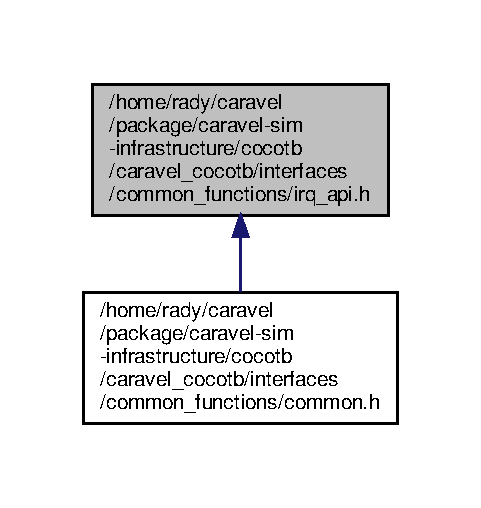
\includegraphics[width=260pt]{irq__api_8h__dep__incl}
\end{center}
\end{figure}
\subsection*{Functions}
\begin{DoxyCompactItemize}
\item 
void \hyperlink{irq__api_8h_a21341597fad3b92332d60feaa5ceaf01}{enable\+\_\+external1\+\_\+irq} (bool is\+\_\+enable)
\item 
void \hyperlink{irq__api_8h_ae059d78d8da468ca24d853d9d573d1f6}{enable\+\_\+external2\+\_\+irq} (bool is\+\_\+enable)
\item 
void \hyperlink{irq__api_8h_a5b50d14e7052f6375664a542de0b869b}{enable\+\_\+timer0\+\_\+irq} (bool is\+\_\+enable)
\item 
void \hyperlink{irq__api_8h_afc59d7e9a7bdac60111985d56dcc7187}{enable\+\_\+uart\+\_\+tx\+\_\+irq} (bool is\+\_\+enable)
\item 
void \hyperlink{irq__api_8h_a96f7a3547cfb0c10cd43d3cb21d297b8}{enable\+\_\+uart\+\_\+rx\+\_\+irq} (bool is\+\_\+enable)
\item 
void \hyperlink{irq__api_8h_aaf1679fd3e37519e4024ae3d8de8a0c2}{enable\+\_\+hk\+\_\+spi\+\_\+irq} (bool is\+\_\+enable)
\end{DoxyCompactItemize}


\subsection{Function Documentation}
\mbox{\Hypertarget{irq__api_8h_a21341597fad3b92332d60feaa5ceaf01}\label{irq__api_8h_a21341597fad3b92332d60feaa5ceaf01}} 
\index{irq\+\_\+api.\+h@{irq\+\_\+api.\+h}!enable\+\_\+external1\+\_\+irq@{enable\+\_\+external1\+\_\+irq}}
\index{enable\+\_\+external1\+\_\+irq@{enable\+\_\+external1\+\_\+irq}!irq\+\_\+api.\+h@{irq\+\_\+api.\+h}}
\subsubsection{\texorpdfstring{enable\+\_\+external1\+\_\+irq()}{enable\_external1\_irq()}}
{\footnotesize\ttfamily void enable\+\_\+external1\+\_\+irq (\begin{DoxyParamCaption}\item[{bool}]{is\+\_\+enable }\end{DoxyParamCaption})}

Enable or disable external1 interrupt G\+P\+IO\mbox{[}7\mbox{]}


\begin{DoxyParams}{Parameters}
{\em is\+\_\+enable} & when 1 (true) interrupt is active and firmware would detect if happened, 0 (false) interrupt is disabled and firmware would not detect if happened \\
\hline
\end{DoxyParams}
\mbox{\Hypertarget{irq__api_8h_ae059d78d8da468ca24d853d9d573d1f6}\label{irq__api_8h_ae059d78d8da468ca24d853d9d573d1f6}} 
\index{irq\+\_\+api.\+h@{irq\+\_\+api.\+h}!enable\+\_\+external2\+\_\+irq@{enable\+\_\+external2\+\_\+irq}}
\index{enable\+\_\+external2\+\_\+irq@{enable\+\_\+external2\+\_\+irq}!irq\+\_\+api.\+h@{irq\+\_\+api.\+h}}
\subsubsection{\texorpdfstring{enable\+\_\+external2\+\_\+irq()}{enable\_external2\_irq()}}
{\footnotesize\ttfamily void enable\+\_\+external2\+\_\+irq (\begin{DoxyParamCaption}\item[{bool}]{is\+\_\+enable }\end{DoxyParamCaption})}

Enable or disable external2 interrupt G\+P\+IO\mbox{[}12\mbox{]}


\begin{DoxyParams}{Parameters}
{\em is\+\_\+enable} & when 1 (true) interrupt is active and firmware would detect if happened, 0 (false) interrupt is disabled and firmware would not detect if happened \\
\hline
\end{DoxyParams}
\mbox{\Hypertarget{irq__api_8h_aaf1679fd3e37519e4024ae3d8de8a0c2}\label{irq__api_8h_aaf1679fd3e37519e4024ae3d8de8a0c2}} 
\index{irq\+\_\+api.\+h@{irq\+\_\+api.\+h}!enable\+\_\+hk\+\_\+spi\+\_\+irq@{enable\+\_\+hk\+\_\+spi\+\_\+irq}}
\index{enable\+\_\+hk\+\_\+spi\+\_\+irq@{enable\+\_\+hk\+\_\+spi\+\_\+irq}!irq\+\_\+api.\+h@{irq\+\_\+api.\+h}}
\subsubsection{\texorpdfstring{enable\+\_\+hk\+\_\+spi\+\_\+irq()}{enable\_hk\_spi\_irq()}}
{\footnotesize\ttfamily void enable\+\_\+hk\+\_\+spi\+\_\+irq (\begin{DoxyParamCaption}\item[{bool}]{is\+\_\+enable }\end{DoxyParamCaption})}

Enable or disable S\+PI interrupt


\begin{DoxyParams}{Parameters}
{\em is\+\_\+enable} & when 1 (true) interrupt is active and firmware would detect if happened, 0 (false) interrupt is disabled and firmware would not detect if happened \\
\hline
\end{DoxyParams}
\mbox{\Hypertarget{irq__api_8h_a5b50d14e7052f6375664a542de0b869b}\label{irq__api_8h_a5b50d14e7052f6375664a542de0b869b}} 
\index{irq\+\_\+api.\+h@{irq\+\_\+api.\+h}!enable\+\_\+timer0\+\_\+irq@{enable\+\_\+timer0\+\_\+irq}}
\index{enable\+\_\+timer0\+\_\+irq@{enable\+\_\+timer0\+\_\+irq}!irq\+\_\+api.\+h@{irq\+\_\+api.\+h}}
\subsubsection{\texorpdfstring{enable\+\_\+timer0\+\_\+irq()}{enable\_timer0\_irq()}}
{\footnotesize\ttfamily void enable\+\_\+timer0\+\_\+irq (\begin{DoxyParamCaption}\item[{bool}]{is\+\_\+enable }\end{DoxyParamCaption})}

Enable or disable timer0 interrupt


\begin{DoxyParams}{Parameters}
{\em is\+\_\+enable} & when 1 (true) interrupt is active and firmware would detect if happened, 0 (false) interrupt is disabled and firmware would not detect if happened \\
\hline
\end{DoxyParams}
\mbox{\Hypertarget{irq__api_8h_a96f7a3547cfb0c10cd43d3cb21d297b8}\label{irq__api_8h_a96f7a3547cfb0c10cd43d3cb21d297b8}} 
\index{irq\+\_\+api.\+h@{irq\+\_\+api.\+h}!enable\+\_\+uart\+\_\+rx\+\_\+irq@{enable\+\_\+uart\+\_\+rx\+\_\+irq}}
\index{enable\+\_\+uart\+\_\+rx\+\_\+irq@{enable\+\_\+uart\+\_\+rx\+\_\+irq}!irq\+\_\+api.\+h@{irq\+\_\+api.\+h}}
\subsubsection{\texorpdfstring{enable\+\_\+uart\+\_\+rx\+\_\+irq()}{enable\_uart\_rx\_irq()}}
{\footnotesize\ttfamily void enable\+\_\+uart\+\_\+rx\+\_\+irq (\begin{DoxyParamCaption}\item[{bool}]{is\+\_\+enable }\end{DoxyParamCaption})}

Enable or disable U\+A\+RT rx interrupt


\begin{DoxyParams}{Parameters}
{\em is\+\_\+enable} & when 1 (true) interrupt is active and firmware would detect if happened, 0 (false) interrupt is disabled and firmware would not detect if happened \\
\hline
\end{DoxyParams}
\mbox{\Hypertarget{irq__api_8h_afc59d7e9a7bdac60111985d56dcc7187}\label{irq__api_8h_afc59d7e9a7bdac60111985d56dcc7187}} 
\index{irq\+\_\+api.\+h@{irq\+\_\+api.\+h}!enable\+\_\+uart\+\_\+tx\+\_\+irq@{enable\+\_\+uart\+\_\+tx\+\_\+irq}}
\index{enable\+\_\+uart\+\_\+tx\+\_\+irq@{enable\+\_\+uart\+\_\+tx\+\_\+irq}!irq\+\_\+api.\+h@{irq\+\_\+api.\+h}}
\subsubsection{\texorpdfstring{enable\+\_\+uart\+\_\+tx\+\_\+irq()}{enable\_uart\_tx\_irq()}}
{\footnotesize\ttfamily void enable\+\_\+uart\+\_\+tx\+\_\+irq (\begin{DoxyParamCaption}\item[{bool}]{is\+\_\+enable }\end{DoxyParamCaption})}

Enable or disable U\+A\+RT tx interrupt


\begin{DoxyParams}{Parameters}
{\em is\+\_\+enable} & when 1 (true) interrupt is active and firmware would detect if happened, 0 (false) interrupt is disabled and firmware would not detect if happened \\
\hline
\end{DoxyParams}

\hypertarget{la_8h}{}\section{/home/rady/caravel/swift/caravel-\/dynamic-\/sims/cocotb/tests/common\+\_\+functions/la.h File Reference}
\label{la_8h}\index{/home/rady/caravel/swift/caravel-\/dynamic-\/sims/cocotb/tests/common\+\_\+functions/la.\+h@{/home/rady/caravel/swift/caravel-\/dynamic-\/sims/cocotb/tests/common\+\_\+functions/la.\+h}}
This graph shows which files directly or indirectly include this file\+:\nopagebreak
\begin{figure}[H]
\begin{center}
\leavevmode
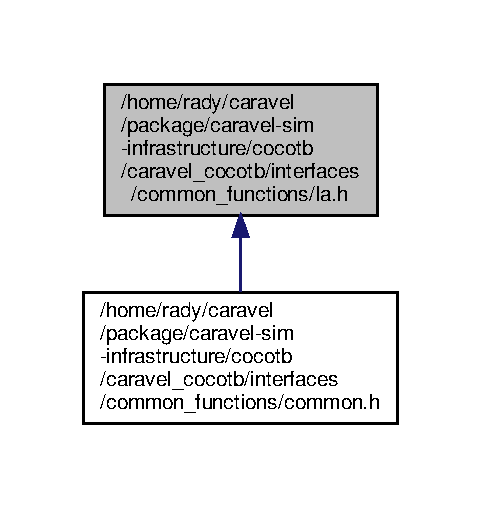
\includegraphics[width=218pt]{la_8h__dep__incl}
\end{center}
\end{figure}
\subsection*{Enumerations}
\begin{DoxyCompactItemize}
\item 
enum \hyperlink{la_8h_a4f5936f125c6714bbd6b3747270f48f0}{la\+\_\+reg\+\_\+number} 
\end{DoxyCompactItemize}
\subsection*{Functions}
\begin{DoxyCompactItemize}
\item 
void \hyperlink{la_8h_aa59af651665d8938229016610ffeb925}{set\+\_\+la\+\_\+ien} (enum \hyperlink{la_8h_a4f5936f125c6714bbd6b3747270f48f0}{la\+\_\+reg\+\_\+number} reg\+\_\+num, unsigned int is\+\_\+enable)
\item 
void \hyperlink{la_8h_aeed29349be1ae153fde34d62a59b9dfc}{set\+\_\+la\+\_\+oen} (enum \hyperlink{la_8h_a4f5936f125c6714bbd6b3747270f48f0}{la\+\_\+reg\+\_\+number} reg\+\_\+num, unsigned int is\+\_\+enable)
\item 
void \hyperlink{la_8h_a8f614c8578907a47d6826cc8cdb6f1d5}{set\+\_\+la\+\_\+reg} (enum \hyperlink{la_8h_a4f5936f125c6714bbd6b3747270f48f0}{la\+\_\+reg\+\_\+number} reg\+\_\+num, unsigned int data)
\item 
unsigned int \hyperlink{la_8h_a46f839584a4aa3a3c0a24a103f8e5a1e}{get\+\_\+la\+\_\+reg} (enum \hyperlink{la_8h_a4f5936f125c6714bbd6b3747270f48f0}{la\+\_\+reg\+\_\+number} reg\+\_\+num)
\end{DoxyCompactItemize}


\subsection{Enumeration Type Documentation}
\mbox{\Hypertarget{la_8h_a4f5936f125c6714bbd6b3747270f48f0}\label{la_8h_a4f5936f125c6714bbd6b3747270f48f0}} 
\index{la.\+h@{la.\+h}!la\+\_\+reg\+\_\+number@{la\+\_\+reg\+\_\+number}}
\index{la\+\_\+reg\+\_\+number@{la\+\_\+reg\+\_\+number}!la.\+h@{la.\+h}}
\subsubsection{\texorpdfstring{la\+\_\+reg\+\_\+number}{la\_reg\_number}}
{\footnotesize\ttfamily enum \hyperlink{la_8h_a4f5936f125c6714bbd6b3747270f48f0}{la\+\_\+reg\+\_\+number}}

Logic analyzers registers \hypertarget{user__addr__space_8h_multi_row}{}
\tabulinesep=1mm
\begin{longtabu} spread 0pt [c]{*{3}{|X[-1]}|}
\caption{Enumerator la\+\_\+reg\+\_\+number}\label{user__addr__space_8h_multi_row}\\
\hline
\rowcolor{\tableheadbgcolor}\textbf{ name}&\textbf{ value}&\textbf{ description }\\\cline{1-3}
\endfirsthead
\hline
\endfoot
\hline
\rowcolor{\tableheadbgcolor}\textbf{ name}&\textbf{ value}&\textbf{ description }\\\cline{1-3}
\endhead
L\+A\+\_\+\+R\+E\+G\+\_\+0&0&First LA register probs \mbox{[}31\+:0\mbox{]} \\\cline{1-3}
L\+A\+\_\+\+R\+E\+G\+\_\+1&1&Second LA register probs \mbox{[}63\+:32\mbox{]} \\\cline{1-3}
L\+A\+\_\+\+R\+E\+G\+\_\+2&2&Third LA register probs \mbox{[}95\+:64\mbox{]} \\\cline{1-3}
L\+A\+\_\+\+R\+E\+G\+\_\+3&3&Fourth LA register probs \mbox{[}95\+:64\mbox{]} \\\cline{1-3}
\end{longtabu}


\subsection{Function Documentation}
\mbox{\Hypertarget{la_8h_a46f839584a4aa3a3c0a24a103f8e5a1e}\label{la_8h_a46f839584a4aa3a3c0a24a103f8e5a1e}} 
\index{la.\+h@{la.\+h}!get\+\_\+la\+\_\+reg@{get\+\_\+la\+\_\+reg}}
\index{get\+\_\+la\+\_\+reg@{get\+\_\+la\+\_\+reg}!la.\+h@{la.\+h}}
\subsubsection{\texorpdfstring{get\+\_\+la\+\_\+reg()}{get\_la\_reg()}}
{\footnotesize\ttfamily unsigned int get\+\_\+la\+\_\+reg (\begin{DoxyParamCaption}\item[{enum \hyperlink{la_8h_a4f5936f125c6714bbd6b3747270f48f0}{la\+\_\+reg\+\_\+number}}]{reg\+\_\+num }\end{DoxyParamCaption})}

Read data through logic analyzers from user project to software

\begin{DoxyNote}{Note}
For this to work correctly probe should be configured as output
\end{DoxyNote}

\begin{DoxyParams}{Parameters}
{\em reg\+\_\+num} & logic analyzer register to read from. Usually not all caravel versions has the same numbers of LA registers They might have 4 registers (128 probs between software and user project) or registers (64 probs between software and user project) \\
\hline
\end{DoxyParams}
\mbox{\Hypertarget{la_8h_aa59af651665d8938229016610ffeb925}\label{la_8h_aa59af651665d8938229016610ffeb925}} 
\index{la.\+h@{la.\+h}!set\+\_\+la\+\_\+ien@{set\+\_\+la\+\_\+ien}}
\index{set\+\_\+la\+\_\+ien@{set\+\_\+la\+\_\+ien}!la.\+h@{la.\+h}}
\subsubsection{\texorpdfstring{set\+\_\+la\+\_\+ien()}{set\_la\_ien()}}
{\footnotesize\ttfamily void set\+\_\+la\+\_\+ien (\begin{DoxyParamCaption}\item[{enum \hyperlink{la_8h_a4f5936f125c6714bbd6b3747270f48f0}{la\+\_\+reg\+\_\+number}}]{reg\+\_\+num,  }\item[{unsigned int}]{is\+\_\+enable }\end{DoxyParamCaption})}

Setting logic analyzer input enable

Enable as input to the user project. Software sends to user project


\begin{DoxyParams}{Parameters}
{\em reg\+\_\+num} & logic analyzer register to write to. Usually not all caravel versions has the same numbers of LA registers They might have 4 registers (128 probs between software and user project) or registers (64 probs between software and user project)\\
\hline
{\em is\+\_\+enable} & 32 bits each bit indicate if the corresponding probe enabled as input \\
\hline
\end{DoxyParams}
\mbox{\Hypertarget{la_8h_aeed29349be1ae153fde34d62a59b9dfc}\label{la_8h_aeed29349be1ae153fde34d62a59b9dfc}} 
\index{la.\+h@{la.\+h}!set\+\_\+la\+\_\+oen@{set\+\_\+la\+\_\+oen}}
\index{set\+\_\+la\+\_\+oen@{set\+\_\+la\+\_\+oen}!la.\+h@{la.\+h}}
\subsubsection{\texorpdfstring{set\+\_\+la\+\_\+oen()}{set\_la\_oen()}}
{\footnotesize\ttfamily void set\+\_\+la\+\_\+oen (\begin{DoxyParamCaption}\item[{enum \hyperlink{la_8h_a4f5936f125c6714bbd6b3747270f48f0}{la\+\_\+reg\+\_\+number}}]{reg\+\_\+num,  }\item[{unsigned int}]{is\+\_\+enable }\end{DoxyParamCaption})}

Setting logic analyzer output enable

Enable as output from the user project. Software receives from user project


\begin{DoxyParams}{Parameters}
{\em reg\+\_\+num} & logic analyzer register to write to. Usually not all caravel versions has the same numbers of LA registers They might have 4 registers (128 probs between software and user project) or registers (64 probs between software and user project)\\
\hline
{\em is\+\_\+enable} & 32 bits each bit indicate if the corresponding probe enabled as output \\
\hline
\end{DoxyParams}
\mbox{\Hypertarget{la_8h_a8f614c8578907a47d6826cc8cdb6f1d5}\label{la_8h_a8f614c8578907a47d6826cc8cdb6f1d5}} 
\index{la.\+h@{la.\+h}!set\+\_\+la\+\_\+reg@{set\+\_\+la\+\_\+reg}}
\index{set\+\_\+la\+\_\+reg@{set\+\_\+la\+\_\+reg}!la.\+h@{la.\+h}}
\subsubsection{\texorpdfstring{set\+\_\+la\+\_\+reg()}{set\_la\_reg()}}
{\footnotesize\ttfamily void set\+\_\+la\+\_\+reg (\begin{DoxyParamCaption}\item[{enum \hyperlink{la_8h_a4f5936f125c6714bbd6b3747270f48f0}{la\+\_\+reg\+\_\+number}}]{reg\+\_\+num,  }\item[{unsigned int}]{data }\end{DoxyParamCaption})}

Write data through logic analyzers from software to user project

\begin{DoxyNote}{Note}
For this to work correctly probe should be configured as output
\end{DoxyNote}

\begin{DoxyParams}{Parameters}
{\em reg\+\_\+num} & logic analyzer register to write to. Usually not all caravel versions has the same numbers of LA registers They might have 4 registers (128 probs between software and user project) or registers (64 probs between software and user project)\\
\hline
{\em data} & data to write through logic analyzers \\
\hline
\end{DoxyParams}

\hypertarget{mgmt__gpio_8h}{}\section{/home/rady/caravel/package/caravel-\/sim-\/infrastructure/cocotb/caravel\+\_\+cocotb/interfaces/common\+\_\+functions/mgmt\+\_\+gpio.h File Reference}
\label{mgmt__gpio_8h}\index{/home/rady/caravel/package/caravel-\/sim-\/infrastructure/cocotb/caravel\+\_\+cocotb/interfaces/common\+\_\+functions/mgmt\+\_\+gpio.\+h@{/home/rady/caravel/package/caravel-\/sim-\/infrastructure/cocotb/caravel\+\_\+cocotb/interfaces/common\+\_\+functions/mgmt\+\_\+gpio.\+h}}
This graph shows which files directly or indirectly include this file\+:\nopagebreak
\begin{figure}[H]
\begin{center}
\leavevmode
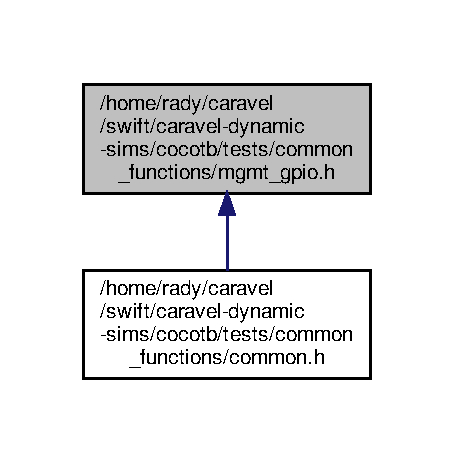
\includegraphics[width=241pt]{mgmt__gpio_8h__dep__incl}
\end{center}
\end{figure}
\subsection*{Functions}
\begin{DoxyCompactItemize}
\item 
void \hyperlink{mgmt__gpio_8h_aebb9ca3b8c8add0a6fdc5d1645a58852}{Managment\+Gpio\+\_\+input\+Enable} ()
\item 
void \hyperlink{mgmt__gpio_8h_a8e72568036b795c978c158b5c0bbd910}{Managment\+Gpio\+\_\+output\+Enable} ()
\item 
void \hyperlink{mgmt__gpio_8h_ad8433f94009bba5dfa1472264ab3f405}{Managment\+Gpio\+\_\+io\+Enable} ()
\item 
void \hyperlink{mgmt__gpio_8h_ab0d97f495e70deeb0261a968f4d83766}{Managment\+Gpio\+\_\+disable} ()
\item 
void \hyperlink{mgmt__gpio_8h_a76f7edf361e9b50ac1f91b3a2efb6d83}{Managment\+Gpio\+\_\+write} (bool data)
\item 
int \hyperlink{mgmt__gpio_8h_a1deb38550709ec95b75b81351aa97f6c}{Managment\+Gpio\+\_\+read} ()
\item 
void \hyperlink{mgmt__gpio_8h_a7f368859e2df2c12ca3c5000f8a19132}{Managment\+Gpio\+\_\+wait} (bool data)
\end{DoxyCompactItemize}


\subsection{Function Documentation}
\mbox{\Hypertarget{mgmt__gpio_8h_ab0d97f495e70deeb0261a968f4d83766}\label{mgmt__gpio_8h_ab0d97f495e70deeb0261a968f4d83766}} 
\index{mgmt\+\_\+gpio.\+h@{mgmt\+\_\+gpio.\+h}!Managment\+Gpio\+\_\+disable@{Managment\+Gpio\+\_\+disable}}
\index{Managment\+Gpio\+\_\+disable@{Managment\+Gpio\+\_\+disable}!mgmt\+\_\+gpio.\+h@{mgmt\+\_\+gpio.\+h}}
\subsubsection{\texorpdfstring{Managment\+Gpio\+\_\+disable()}{ManagmentGpio\_disable()}}
{\footnotesize\ttfamily void Managment\+Gpio\+\_\+disable (\begin{DoxyParamCaption}{ }\end{DoxyParamCaption})}

Configure management G\+P\+IO as floating It\textquotesingle{}s not connected as input or output \mbox{\Hypertarget{mgmt__gpio_8h_aebb9ca3b8c8add0a6fdc5d1645a58852}\label{mgmt__gpio_8h_aebb9ca3b8c8add0a6fdc5d1645a58852}} 
\index{mgmt\+\_\+gpio.\+h@{mgmt\+\_\+gpio.\+h}!Managment\+Gpio\+\_\+input\+Enable@{Managment\+Gpio\+\_\+input\+Enable}}
\index{Managment\+Gpio\+\_\+input\+Enable@{Managment\+Gpio\+\_\+input\+Enable}!mgmt\+\_\+gpio.\+h@{mgmt\+\_\+gpio.\+h}}
\subsubsection{\texorpdfstring{Managment\+Gpio\+\_\+input\+Enable()}{ManagmentGpio\_inputEnable()}}
{\footnotesize\ttfamily void Managment\+Gpio\+\_\+input\+Enable (\begin{DoxyParamCaption}{ }\end{DoxyParamCaption})}

Configure management G\+P\+IO as input \mbox{\Hypertarget{mgmt__gpio_8h_ad8433f94009bba5dfa1472264ab3f405}\label{mgmt__gpio_8h_ad8433f94009bba5dfa1472264ab3f405}} 
\index{mgmt\+\_\+gpio.\+h@{mgmt\+\_\+gpio.\+h}!Managment\+Gpio\+\_\+io\+Enable@{Managment\+Gpio\+\_\+io\+Enable}}
\index{Managment\+Gpio\+\_\+io\+Enable@{Managment\+Gpio\+\_\+io\+Enable}!mgmt\+\_\+gpio.\+h@{mgmt\+\_\+gpio.\+h}}
\subsubsection{\texorpdfstring{Managment\+Gpio\+\_\+io\+Enable()}{ManagmentGpio\_ioEnable()}}
{\footnotesize\ttfamily void Managment\+Gpio\+\_\+io\+Enable (\begin{DoxyParamCaption}{ }\end{DoxyParamCaption})}

Configure management G\+P\+IO as bi-\/direction \mbox{\Hypertarget{mgmt__gpio_8h_a8e72568036b795c978c158b5c0bbd910}\label{mgmt__gpio_8h_a8e72568036b795c978c158b5c0bbd910}} 
\index{mgmt\+\_\+gpio.\+h@{mgmt\+\_\+gpio.\+h}!Managment\+Gpio\+\_\+output\+Enable@{Managment\+Gpio\+\_\+output\+Enable}}
\index{Managment\+Gpio\+\_\+output\+Enable@{Managment\+Gpio\+\_\+output\+Enable}!mgmt\+\_\+gpio.\+h@{mgmt\+\_\+gpio.\+h}}
\subsubsection{\texorpdfstring{Managment\+Gpio\+\_\+output\+Enable()}{ManagmentGpio\_outputEnable()}}
{\footnotesize\ttfamily void Managment\+Gpio\+\_\+output\+Enable (\begin{DoxyParamCaption}{ }\end{DoxyParamCaption})}

Configure management G\+P\+IO as output \mbox{\Hypertarget{mgmt__gpio_8h_a1deb38550709ec95b75b81351aa97f6c}\label{mgmt__gpio_8h_a1deb38550709ec95b75b81351aa97f6c}} 
\index{mgmt\+\_\+gpio.\+h@{mgmt\+\_\+gpio.\+h}!Managment\+Gpio\+\_\+read@{Managment\+Gpio\+\_\+read}}
\index{Managment\+Gpio\+\_\+read@{Managment\+Gpio\+\_\+read}!mgmt\+\_\+gpio.\+h@{mgmt\+\_\+gpio.\+h}}
\subsubsection{\texorpdfstring{Managment\+Gpio\+\_\+read()}{ManagmentGpio\_read()}}
{\footnotesize\ttfamily int Managment\+Gpio\+\_\+read (\begin{DoxyParamCaption}{ }\end{DoxyParamCaption})}

Read data in management G\+P\+IO

\begin{DoxyNote}{Note}
This function works correctly when management G\+P\+IO configured as input If management doesn\textquotesingle{}t connect to anything the firmware would read \char`\"{}0\char`\"{} 
\end{DoxyNote}
\mbox{\Hypertarget{mgmt__gpio_8h_a7f368859e2df2c12ca3c5000f8a19132}\label{mgmt__gpio_8h_a7f368859e2df2c12ca3c5000f8a19132}} 
\index{mgmt\+\_\+gpio.\+h@{mgmt\+\_\+gpio.\+h}!Managment\+Gpio\+\_\+wait@{Managment\+Gpio\+\_\+wait}}
\index{Managment\+Gpio\+\_\+wait@{Managment\+Gpio\+\_\+wait}!mgmt\+\_\+gpio.\+h@{mgmt\+\_\+gpio.\+h}}
\subsubsection{\texorpdfstring{Managment\+Gpio\+\_\+wait()}{ManagmentGpio\_wait()}}
{\footnotesize\ttfamily void Managment\+Gpio\+\_\+wait (\begin{DoxyParamCaption}\item[{bool}]{data }\end{DoxyParamCaption})}

Wait over management G\+P\+IO to equal data

\begin{DoxyNote}{Note}
This function works correctly when management G\+P\+IO configured as input
\end{DoxyNote}

\begin{DoxyParams}{Parameters}
{\em data} & data to wait over \\
\hline
\end{DoxyParams}
\mbox{\Hypertarget{mgmt__gpio_8h_a76f7edf361e9b50ac1f91b3a2efb6d83}\label{mgmt__gpio_8h_a76f7edf361e9b50ac1f91b3a2efb6d83}} 
\index{mgmt\+\_\+gpio.\+h@{mgmt\+\_\+gpio.\+h}!Managment\+Gpio\+\_\+write@{Managment\+Gpio\+\_\+write}}
\index{Managment\+Gpio\+\_\+write@{Managment\+Gpio\+\_\+write}!mgmt\+\_\+gpio.\+h@{mgmt\+\_\+gpio.\+h}}
\subsubsection{\texorpdfstring{Managment\+Gpio\+\_\+write()}{ManagmentGpio\_write()}}
{\footnotesize\ttfamily void Managment\+Gpio\+\_\+write (\begin{DoxyParamCaption}\item[{bool}]{data }\end{DoxyParamCaption})}

Write data in management G\+P\+IO


\begin{DoxyParams}{Parameters}
{\em data} & data to write at management G\+P\+IO possible values are 0 and 1\\
\hline
\end{DoxyParams}
\begin{DoxyNote}{Note}
This function works when management G\+P\+IO configured as output 
\end{DoxyNote}

\hypertarget{spi__master_8h}{}\section{/home/rady/caravel/caravel\+\_\+release/caravel-\/dynamic-\/sims/cocotb/interfaces/common\+\_\+functions/spi\+\_\+master.h File Reference}
\label{spi__master_8h}\index{/home/rady/caravel/caravel\+\_\+release/caravel-\/dynamic-\/sims/cocotb/interfaces/common\+\_\+functions/spi\+\_\+master.\+h@{/home/rady/caravel/caravel\+\_\+release/caravel-\/dynamic-\/sims/cocotb/interfaces/common\+\_\+functions/spi\+\_\+master.\+h}}
This graph shows which files directly or indirectly include this file\+:\nopagebreak
\begin{figure}[H]
\begin{center}
\leavevmode
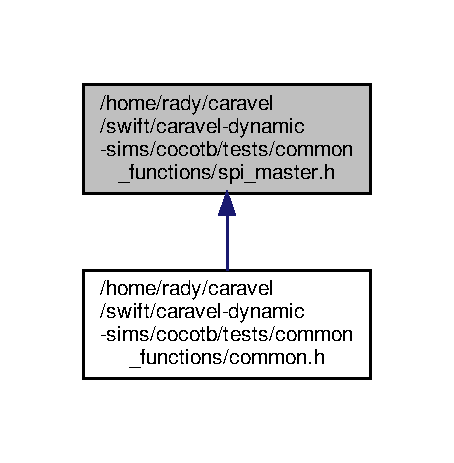
\includegraphics[width=241pt]{spi__master_8h__dep__incl}
\end{center}
\end{figure}
\subsection*{Functions}
\begin{DoxyCompactItemize}
\item 
void \hyperlink{spi__master_8h_ac256606f0178011ddb85162d9584c487}{spi\+\_\+write} (char c)
\item 
char \hyperlink{spi__master_8h_ae677e13a3b0995516e495ced349dbcc5}{spi\+\_\+read} ()
\item 
void \hyperlink{spi__master_8h_a60653a00868af39a2ae44b05717197d5}{enable\+\_\+spi} (bool is\+\_\+enable)
\item 
void \hyperlink{spi__master_8h_a904d489d359261aab3e5149f4ac4fb0f}{enable\+\_\+\+CS} (bool is\+\_\+enable)
\end{DoxyCompactItemize}


\subsection{Function Documentation}
\mbox{\Hypertarget{spi__master_8h_a904d489d359261aab3e5149f4ac4fb0f}\label{spi__master_8h_a904d489d359261aab3e5149f4ac4fb0f}} 
\index{spi\+\_\+master.\+h@{spi\+\_\+master.\+h}!enable\+\_\+\+CS@{enable\+\_\+\+CS}}
\index{enable\+\_\+\+CS@{enable\+\_\+\+CS}!spi\+\_\+master.\+h@{spi\+\_\+master.\+h}}
\subsubsection{\texorpdfstring{enable\+\_\+\+C\+S()}{enable\_CS()}}
{\footnotesize\ttfamily void enable\+\_\+\+CS (\begin{DoxyParamCaption}\item[{bool}]{is\+\_\+enable }\end{DoxyParamCaption})}

assert or deassert chip select


\begin{DoxyParams}{Parameters}
{\em is\+\_\+enable} & when 1 (true) chip select is asserted, 0 (false) chip select is deasserted \\
\hline
\end{DoxyParams}
\mbox{\Hypertarget{spi__master_8h_a60653a00868af39a2ae44b05717197d5}\label{spi__master_8h_a60653a00868af39a2ae44b05717197d5}} 
\index{spi\+\_\+master.\+h@{spi\+\_\+master.\+h}!enable\+\_\+spi@{enable\+\_\+spi}}
\index{enable\+\_\+spi@{enable\+\_\+spi}!spi\+\_\+master.\+h@{spi\+\_\+master.\+h}}
\subsubsection{\texorpdfstring{enable\+\_\+spi()}{enable\_spi()}}
{\footnotesize\ttfamily void enable\+\_\+spi (\begin{DoxyParamCaption}\item[{bool}]{is\+\_\+enable }\end{DoxyParamCaption})}

Enable or disable the master S\+PI


\begin{DoxyParams}{Parameters}
{\em is\+\_\+enable} & when 1 (true) master S\+PI is active, 0 (false) master S\+PI is disabled \\
\hline
\end{DoxyParams}
\mbox{\Hypertarget{spi__master_8h_ae677e13a3b0995516e495ced349dbcc5}\label{spi__master_8h_ae677e13a3b0995516e495ced349dbcc5}} 
\index{spi\+\_\+master.\+h@{spi\+\_\+master.\+h}!spi\+\_\+read@{spi\+\_\+read}}
\index{spi\+\_\+read@{spi\+\_\+read}!spi\+\_\+master.\+h@{spi\+\_\+master.\+h}}
\subsubsection{\texorpdfstring{spi\+\_\+read()}{spi\_read()}}
{\footnotesize\ttfamily char spi\+\_\+read (\begin{DoxyParamCaption}{ }\end{DoxyParamCaption})}

Read byte (8bits) through S\+PI master \mbox{\Hypertarget{spi__master_8h_ac256606f0178011ddb85162d9584c487}\label{spi__master_8h_ac256606f0178011ddb85162d9584c487}} 
\index{spi\+\_\+master.\+h@{spi\+\_\+master.\+h}!spi\+\_\+write@{spi\+\_\+write}}
\index{spi\+\_\+write@{spi\+\_\+write}!spi\+\_\+master.\+h@{spi\+\_\+master.\+h}}
\subsubsection{\texorpdfstring{spi\+\_\+write()}{spi\_write()}}
{\footnotesize\ttfamily void spi\+\_\+write (\begin{DoxyParamCaption}\item[{char}]{c }\end{DoxyParamCaption})}

Write byte (8bits) through S\+PI master


\begin{DoxyParams}{Parameters}
{\em c} & byte to write range 0x0 to 0x\+FF \\
\hline
\end{DoxyParams}

\hypertarget{timer0_8h}{}\section{/home/rady/caravel/caravel\+\_\+user\+\_\+project/caravel-\/sim-\/infrastructure/cocotb/interfaces/common\+\_\+functions/timer0.h File Reference}
\label{timer0_8h}\index{/home/rady/caravel/caravel\+\_\+user\+\_\+project/caravel-\/sim-\/infrastructure/cocotb/interfaces/common\+\_\+functions/timer0.\+h@{/home/rady/caravel/caravel\+\_\+user\+\_\+project/caravel-\/sim-\/infrastructure/cocotb/interfaces/common\+\_\+functions/timer0.\+h}}
This graph shows which files directly or indirectly include this file\+:
\nopagebreak
\begin{figure}[H]
\begin{center}
\leavevmode
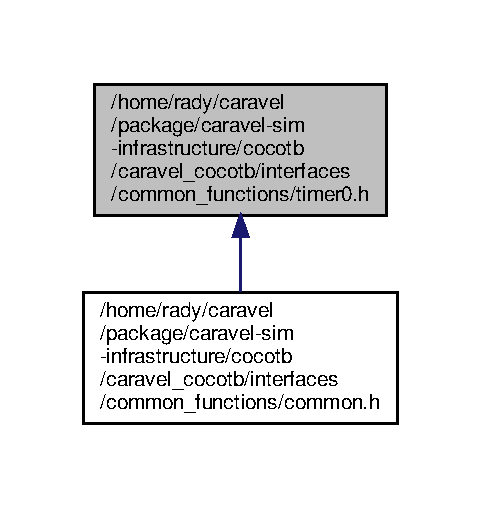
\includegraphics[width=215pt]{timer0_8h__dep__incl}
\end{center}
\end{figure}
\subsection*{Functions}
\begin{DoxyCompactItemize}
\item 
void \hyperlink{timer0_8h_a618b157336f2fbb272590e57b0105fb4}{timer0\+\_\+oneshot\+\_\+configure} (unsigned int count)
\item 
void \hyperlink{timer0_8h_ace0a359a15e1744a3f8eb4e8a415680e}{timer0\+\_\+periodic\+\_\+configure} (unsigned int count)
\item 
void \hyperlink{timer0_8h_aed97be9effff00e8469940bbac4cac53}{enable\+\_\+timer0} (bool is\+\_\+enable)
\item 
unsigned int \hyperlink{timer0_8h_a4b344afe9da30e277cbcc840cec73067}{get\+\_\+timer0\+\_\+val} ()
\end{DoxyCompactItemize}


\subsection{Function Documentation}
\mbox{\Hypertarget{timer0_8h_aed97be9effff00e8469940bbac4cac53}\label{timer0_8h_aed97be9effff00e8469940bbac4cac53}} 
\index{timer0.\+h@{timer0.\+h}!enable\+\_\+timer0@{enable\+\_\+timer0}}
\index{enable\+\_\+timer0@{enable\+\_\+timer0}!timer0.\+h@{timer0.\+h}}
\subsubsection{\texorpdfstring{enable\+\_\+timer0()}{enable\_timer0()}}
{\footnotesize\ttfamily void enable\+\_\+timer0 (\begin{DoxyParamCaption}\item[{bool}]{is\+\_\+enable }\end{DoxyParamCaption})}

Enable or Disable timer0


\begin{DoxyParams}{Parameters}
{\em is\+\_\+enable} & when 1 (true) timer0 is enable (start counting), 0 (false) timer0 is disabled \\
\hline
\end{DoxyParams}
\mbox{\Hypertarget{timer0_8h_a4b344afe9da30e277cbcc840cec73067}\label{timer0_8h_a4b344afe9da30e277cbcc840cec73067}} 
\index{timer0.\+h@{timer0.\+h}!get\+\_\+timer0\+\_\+val@{get\+\_\+timer0\+\_\+val}}
\index{get\+\_\+timer0\+\_\+val@{get\+\_\+timer0\+\_\+val}!timer0.\+h@{timer0.\+h}}
\subsubsection{\texorpdfstring{get\+\_\+timer0\+\_\+val()}{get\_timer0\_val()}}
{\footnotesize\ttfamily unsigned int get\+\_\+timer0\+\_\+val (\begin{DoxyParamCaption}{ }\end{DoxyParamCaption})}

Get timer current value \mbox{\Hypertarget{timer0_8h_a618b157336f2fbb272590e57b0105fb4}\label{timer0_8h_a618b157336f2fbb272590e57b0105fb4}} 
\index{timer0.\+h@{timer0.\+h}!timer0\+\_\+oneshot\+\_\+configure@{timer0\+\_\+oneshot\+\_\+configure}}
\index{timer0\+\_\+oneshot\+\_\+configure@{timer0\+\_\+oneshot\+\_\+configure}!timer0.\+h@{timer0.\+h}}
\subsubsection{\texorpdfstring{timer0\+\_\+oneshot\+\_\+configure()}{timer0\_oneshot\_configure()}}
{\footnotesize\ttfamily void timer0\+\_\+oneshot\+\_\+configure (\begin{DoxyParamCaption}\item[{unsigned int}]{count }\end{DoxyParamCaption})}

Start Timer in oneshot countdown mode start value is count


\begin{DoxyParams}{Parameters}
{\em count} & start value in the counter $>$ 0 \\
\hline
\end{DoxyParams}
\mbox{\Hypertarget{timer0_8h_ace0a359a15e1744a3f8eb4e8a415680e}\label{timer0_8h_ace0a359a15e1744a3f8eb4e8a415680e}} 
\index{timer0.\+h@{timer0.\+h}!timer0\+\_\+periodic\+\_\+configure@{timer0\+\_\+periodic\+\_\+configure}}
\index{timer0\+\_\+periodic\+\_\+configure@{timer0\+\_\+periodic\+\_\+configure}!timer0.\+h@{timer0.\+h}}
\subsubsection{\texorpdfstring{timer0\+\_\+periodic\+\_\+configure()}{timer0\_periodic\_configure()}}
{\footnotesize\ttfamily void timer0\+\_\+periodic\+\_\+configure (\begin{DoxyParamCaption}\item[{unsigned int}]{count }\end{DoxyParamCaption})}

Start counter in periodic countdown mode start value is count

Timer will roll over to the count value when it reaches 0 
\begin{DoxyParams}{Parameters}
{\em count} & start value in the counter $>$ 0 \\
\hline
\end{DoxyParams}

\hypertarget{uart__api_8h}{}\section{/home/rady/caravel/swift/caravel-\/dynamic-\/sims/cocotb/tests/common\+\_\+functions/uart\+\_\+api.h File Reference}
\label{uart__api_8h}\index{/home/rady/caravel/swift/caravel-\/dynamic-\/sims/cocotb/tests/common\+\_\+functions/uart\+\_\+api.\+h@{/home/rady/caravel/swift/caravel-\/dynamic-\/sims/cocotb/tests/common\+\_\+functions/uart\+\_\+api.\+h}}
This graph shows which files directly or indirectly include this file\+:\nopagebreak
\begin{figure}[H]
\begin{center}
\leavevmode
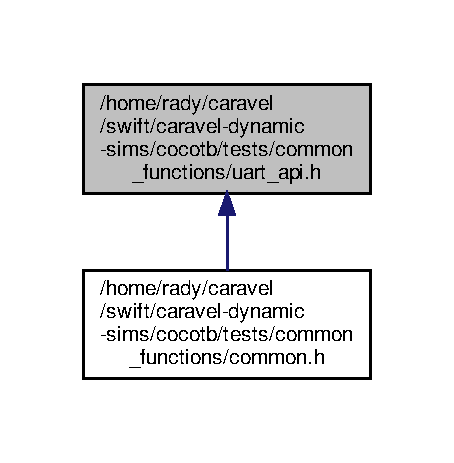
\includegraphics[width=218pt]{uart__api_8h__dep__incl}
\end{center}
\end{figure}
\subsection*{Functions}
\begin{DoxyCompactItemize}
\item 
void \hyperlink{uart__api_8h_af271ffef8910e5c9f6ddf14163ec7e6a}{enable\+\_\+uart\+\_\+\+TX} (bool is\+\_\+enable)
\item 
void \hyperlink{uart__api_8h_a23a72c60afce70b08a0fd3ff45a4f024}{uart\+\_\+\+R\+X\+\_\+enable} (bool is\+\_\+enable)
\item 
char \hyperlink{uart__api_8h_a11508a3c55df6779452e795b23f2af40}{uart\+\_\+getc} ()
\item 
void \hyperlink{uart__api_8h_a8398a7147ed6979b318b895c18766975}{uart\+\_\+pop\+\_\+char} ()
\item 
void \hyperlink{uart__api_8h_a2d0091e019fc1a50c3cc9f4c86dd73c2}{print} (const char $\ast$p)
\end{DoxyCompactItemize}


\subsection{Function Documentation}
\mbox{\Hypertarget{uart__api_8h_af271ffef8910e5c9f6ddf14163ec7e6a}\label{uart__api_8h_af271ffef8910e5c9f6ddf14163ec7e6a}} 
\index{uart\+\_\+api.\+h@{uart\+\_\+api.\+h}!enable\+\_\+uart\+\_\+\+TX@{enable\+\_\+uart\+\_\+\+TX}}
\index{enable\+\_\+uart\+\_\+\+TX@{enable\+\_\+uart\+\_\+\+TX}!uart\+\_\+api.\+h@{uart\+\_\+api.\+h}}
\subsubsection{\texorpdfstring{enable\+\_\+uart\+\_\+\+T\+X()}{enable\_uart\_TX()}}
{\footnotesize\ttfamily void enable\+\_\+uart\+\_\+\+TX (\begin{DoxyParamCaption}\item[{bool}]{is\+\_\+enable }\end{DoxyParamCaption})}

Enable or disable TX of U\+A\+RT


\begin{DoxyParams}{Parameters}
{\em is\+\_\+enable} & when 1(true) U\+A\+RT TX enable, 0 (false) U\+A\+RT TX disable\\
\hline
\end{DoxyParams}
\begin{DoxyNote}{Note}
Some caravel C\+PU enable and disable U\+A\+RT TX and RX together 
\end{DoxyNote}
\mbox{\Hypertarget{uart__api_8h_a2d0091e019fc1a50c3cc9f4c86dd73c2}\label{uart__api_8h_a2d0091e019fc1a50c3cc9f4c86dd73c2}} 
\index{uart\+\_\+api.\+h@{uart\+\_\+api.\+h}!print@{print}}
\index{print@{print}!uart\+\_\+api.\+h@{uart\+\_\+api.\+h}}
\subsubsection{\texorpdfstring{print()}{print()}}
{\footnotesize\ttfamily void print (\begin{DoxyParamCaption}\item[{const char $\ast$}]{p }\end{DoxyParamCaption})}

Send A\+S\+C\+II symbol or symbols through U\+A\+RT

TX mode have to be enabled \mbox{\Hypertarget{uart__api_8h_a11508a3c55df6779452e795b23f2af40}\label{uart__api_8h_a11508a3c55df6779452e795b23f2af40}} 
\index{uart\+\_\+api.\+h@{uart\+\_\+api.\+h}!uart\+\_\+getc@{uart\+\_\+getc}}
\index{uart\+\_\+getc@{uart\+\_\+getc}!uart\+\_\+api.\+h@{uart\+\_\+api.\+h}}
\subsubsection{\texorpdfstring{uart\+\_\+getc()}{uart\_getc()}}
{\footnotesize\ttfamily char uart\+\_\+getc (\begin{DoxyParamCaption}{ }\end{DoxyParamCaption})}

Wait receiving A\+S\+C\+II symbol and return it.

Return the first A\+S\+C\+II symbol of the U\+A\+RT received queue

RX mode have to be enabled \mbox{\Hypertarget{uart__api_8h_a8398a7147ed6979b318b895c18766975}\label{uart__api_8h_a8398a7147ed6979b318b895c18766975}} 
\index{uart\+\_\+api.\+h@{uart\+\_\+api.\+h}!uart\+\_\+pop\+\_\+char@{uart\+\_\+pop\+\_\+char}}
\index{uart\+\_\+pop\+\_\+char@{uart\+\_\+pop\+\_\+char}!uart\+\_\+api.\+h@{uart\+\_\+api.\+h}}
\subsubsection{\texorpdfstring{uart\+\_\+pop\+\_\+char()}{uart\_pop\_char()}}
{\footnotesize\ttfamily void uart\+\_\+pop\+\_\+char (\begin{DoxyParamCaption}{ }\end{DoxyParamCaption})}

Pop the first A\+S\+C\+II symbol of the U\+A\+RT received queue

\hyperlink{uart__api_8h_a11508a3c55df6779452e795b23f2af40}{uart\+\_\+getc()} function would keeping reading the same symbol unless this function is called \mbox{\Hypertarget{uart__api_8h_a23a72c60afce70b08a0fd3ff45a4f024}\label{uart__api_8h_a23a72c60afce70b08a0fd3ff45a4f024}} 
\index{uart\+\_\+api.\+h@{uart\+\_\+api.\+h}!uart\+\_\+\+R\+X\+\_\+enable@{uart\+\_\+\+R\+X\+\_\+enable}}
\index{uart\+\_\+\+R\+X\+\_\+enable@{uart\+\_\+\+R\+X\+\_\+enable}!uart\+\_\+api.\+h@{uart\+\_\+api.\+h}}
\subsubsection{\texorpdfstring{uart\+\_\+\+R\+X\+\_\+enable()}{uart\_RX\_enable()}}
{\footnotesize\ttfamily void uart\+\_\+\+R\+X\+\_\+enable (\begin{DoxyParamCaption}\item[{bool}]{is\+\_\+enable }\end{DoxyParamCaption})}

Enable or disable RX of U\+A\+RT


\begin{DoxyParams}{Parameters}
{\em is\+\_\+enable} & when 1(true) U\+A\+RT RX enable, 0 (false) U\+A\+RT RX disable\\
\hline
\end{DoxyParams}
\begin{DoxyNote}{Note}
Some caravel C\+PU enable and disable U\+A\+RT TX and RX together 
\end{DoxyNote}

\hypertarget{user__addr__space_8h}{}\section{/home/rady/caravel/swift/caravel-\/dynamic-\/sims/cocotb/tests/common\+\_\+functions/user\+\_\+addr\+\_\+space.h File Reference}
\label{user__addr__space_8h}\index{/home/rady/caravel/swift/caravel-\/dynamic-\/sims/cocotb/tests/common\+\_\+functions/user\+\_\+addr\+\_\+space.\+h@{/home/rady/caravel/swift/caravel-\/dynamic-\/sims/cocotb/tests/common\+\_\+functions/user\+\_\+addr\+\_\+space.\+h}}
This graph shows which files directly or indirectly include this file\+:\nopagebreak
\begin{figure}[H]
\begin{center}
\leavevmode
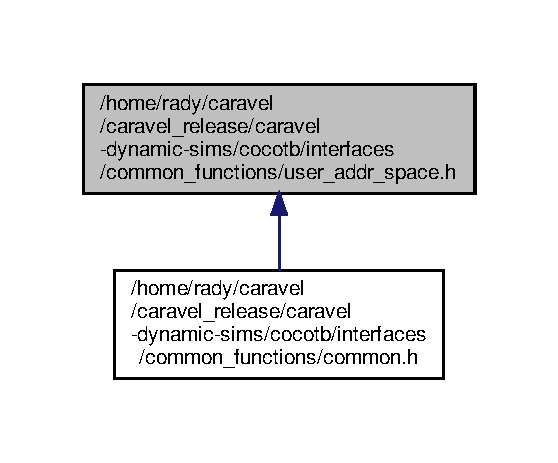
\includegraphics[width=227pt]{user__addr__space_8h__dep__incl}
\end{center}
\end{figure}
\subsection*{Functions}
\begin{DoxyCompactItemize}
\item 
void \hyperlink{user__addr__space_8h_a291884d7ca06f6fc9a1f43a5ef274260}{write\+\_\+user\+\_\+double\+\_\+word} (unsigned int data, int offset)
\item 
unsigned int \hyperlink{user__addr__space_8h_aa9a3f20abb8888d9f06601b96ca8fbae}{read\+\_\+user\+\_\+double\+\_\+word} (int offset)
\item 
void \hyperlink{user__addr__space_8h_ac8c9de3c8721308bc981b0ca98402517}{write\+\_\+user\+\_\+word} (unsigned short data, unsigned int offset, bool is\+\_\+first\+\_\+word)
\item 
unsigned short \hyperlink{user__addr__space_8h_a929692f180f9152c63eef1849e1d15a1}{read\+\_\+user\+\_\+word} (unsigned int offset, bool is\+\_\+first\+\_\+word)
\item 
void \hyperlink{user__addr__space_8h_a0eb906122234d6c9f173c03fe6fd2345}{write\+\_\+user\+\_\+byte} (unsigned char data, unsigned int offset, unsigned char byte\+\_\+num)
\item 
unsigned char \hyperlink{user__addr__space_8h_af2e75a434a8110b6522be2ad1a406713}{read\+\_\+user\+\_\+byte} (unsigned int offset, unsigned char byte\+\_\+num)
\end{DoxyCompactItemize}


\subsection{Function Documentation}
\mbox{\Hypertarget{user__addr__space_8h_af2e75a434a8110b6522be2ad1a406713}\label{user__addr__space_8h_af2e75a434a8110b6522be2ad1a406713}} 
\index{user\+\_\+addr\+\_\+space.\+h@{user\+\_\+addr\+\_\+space.\+h}!read\+\_\+user\+\_\+byte@{read\+\_\+user\+\_\+byte}}
\index{read\+\_\+user\+\_\+byte@{read\+\_\+user\+\_\+byte}!user\+\_\+addr\+\_\+space.\+h@{user\+\_\+addr\+\_\+space.\+h}}
\subsubsection{\texorpdfstring{read\+\_\+user\+\_\+byte()}{read\_user\_byte()}}
{\footnotesize\ttfamily unsigned char read\+\_\+user\+\_\+byte (\begin{DoxyParamCaption}\item[{unsigned int}]{offset,  }\item[{unsigned char}]{byte\+\_\+num }\end{DoxyParamCaption})}

Read byte at user address space 32 bit register


\begin{DoxyParams}{Parameters}
{\em int} & offset the offset of the register to write. Origin at the user project address \\
\hline
{\em byte\+\_\+num} & number of the in the 4byte register (32 bits)\\
\hline
\end{DoxyParams}
\begin{DoxyNote}{Note}
if user space address length is 4 bits address that mean it has 2$^\wedge$4 bytes = 16 bytes. In this case offset would take values from 0 to 3 and byte\+\_\+num can take 0 to 3. ~\newline
Typically address space is 26 address bits which mean it has 67,108,864 bytes. In this case offset would take values from 0 to 16,777,215 and byte\+\_\+num can take 0 or 4.
\end{DoxyNote}
\hypertarget{user__addr__space_8h_multi_row}{}
\tabulinesep=1mm
\begin{longtabu} spread 0pt [c]{*{6}{|X[-1]}|}
\caption{world memory (2byte offset)}\label{user__addr__space_8h_multi_row}\\
\hline
\rowcolor{\tableheadbgcolor}\textbf{ byte\+\_\+num}&\textbf{ -\/}&\textbf{ 0 }&\textbf{ 1}&\textbf{ 2}&\textbf{ 3 }\\\cline{1-6}
\endfirsthead
\hline
\endfoot
\hline
\rowcolor{\tableheadbgcolor}\textbf{ byte\+\_\+num}&\textbf{ -\/}&\textbf{ 0 }&\textbf{ 1}&\textbf{ 2}&\textbf{ 3 }\\\cline{1-6}
\endhead
\rowcolor{\tableheadbgcolor}\textbf{ address}&\textbf{ offset }&\textbf{ byte0}&\textbf{ byte1}&\textbf{ byte2}&\textbf{ byte3 }\\\cline{1-6}
0x0&0&0&1&2&3 \\\cline{1-6}
0x4&1&4&5&6&7 \\\cline{1-6}
0x8&2&8&9&10&11 \\\cline{1-6}
0xC&3&12&13&14&15 \\\cline{1-6}
\end{longtabu}
\mbox{\Hypertarget{user__addr__space_8h_aa9a3f20abb8888d9f06601b96ca8fbae}\label{user__addr__space_8h_aa9a3f20abb8888d9f06601b96ca8fbae}} 
\index{user\+\_\+addr\+\_\+space.\+h@{user\+\_\+addr\+\_\+space.\+h}!read\+\_\+user\+\_\+double\+\_\+word@{read\+\_\+user\+\_\+double\+\_\+word}}
\index{read\+\_\+user\+\_\+double\+\_\+word@{read\+\_\+user\+\_\+double\+\_\+word}!user\+\_\+addr\+\_\+space.\+h@{user\+\_\+addr\+\_\+space.\+h}}
\subsubsection{\texorpdfstring{read\+\_\+user\+\_\+double\+\_\+word()}{read\_user\_double\_word()}}
{\footnotesize\ttfamily unsigned int read\+\_\+user\+\_\+double\+\_\+word (\begin{DoxyParamCaption}\item[{int}]{offset }\end{DoxyParamCaption})}

Read double word (4 bytes) at user address space 32 bit register


\begin{DoxyParams}{Parameters}
{\em offset} & the offset of the register to write. Origin at the user project address\\
\hline
\end{DoxyParams}
\begin{DoxyNote}{Note}
if user space address length is 4 bits address that mean it has 2$^\wedge$4 bytes = 16 bytes that mean it has only 4 doublewords. In this case offset would take values from 0 to 3. ~\newline
 Typically address space is 26 address bits which mean it has 67,108,864 bytes = 16,777,216 doubleword In this case offset would take values from 0 to 16,777,215.
\end{DoxyNote}
\hypertarget{user__addr__space_8h_multi_row}{}
\tabulinesep=1mm
\begin{longtabu} spread 0pt [c]{*{6}{|X[-1]}|}
\caption{double world memory (4byte offset)}\label{user__addr__space_8h_multi_row}\\
\hline
\rowcolor{\tableheadbgcolor}\textbf{ address}&\textbf{ offset }&\textbf{ byte0}&\textbf{ byte1}&\textbf{ byte2}&\textbf{ byte3 }\\\cline{1-6}
\endfirsthead
\hline
\endfoot
\hline
\rowcolor{\tableheadbgcolor}\textbf{ address}&\textbf{ offset }&\textbf{ byte0}&\textbf{ byte1}&\textbf{ byte2}&\textbf{ byte3 }\\\cline{1-6}
\endhead
0x0&0&0&1&2&3 \\\cline{1-6}
0x4&1&4&5&6&7 \\\cline{1-6}
0x8&2&8&9&10&11 \\\cline{1-6}
0xC&3&12&13&14&15 \\\cline{1-6}
\end{longtabu}
\mbox{\Hypertarget{user__addr__space_8h_a929692f180f9152c63eef1849e1d15a1}\label{user__addr__space_8h_a929692f180f9152c63eef1849e1d15a1}} 
\index{user\+\_\+addr\+\_\+space.\+h@{user\+\_\+addr\+\_\+space.\+h}!read\+\_\+user\+\_\+word@{read\+\_\+user\+\_\+word}}
\index{read\+\_\+user\+\_\+word@{read\+\_\+user\+\_\+word}!user\+\_\+addr\+\_\+space.\+h@{user\+\_\+addr\+\_\+space.\+h}}
\subsubsection{\texorpdfstring{read\+\_\+user\+\_\+word()}{read\_user\_word()}}
{\footnotesize\ttfamily unsigned short read\+\_\+user\+\_\+word (\begin{DoxyParamCaption}\item[{unsigned int}]{offset,  }\item[{bool}]{is\+\_\+first\+\_\+word }\end{DoxyParamCaption})}

Read word (2 bytes) at user address space 32 bit register


\begin{DoxyParams}{Parameters}
{\em offset} & the offset of the register to write. Origin at the user project address \\
\hline
{\em is\+\_\+first\+\_\+word} & the offset of the register to write. Origin at the user project address\\
\hline
\end{DoxyParams}
\begin{DoxyNote}{Note}
if user space address length is 4 bits address that mean it has 2$^\wedge$4 bytes = 16 bytes that mean it has only 8 words. In this case offset would take values from 0 to 3 and is\+\_\+first\+\_\+word can take 0 or 1. ~\newline
Typically address space is 26 address bits which mean it has 67,108,864 bytes = 33,554,432 doubleword In this case offset would take values from 0 to 16,777,215 and is\+\_\+first\+\_\+word can take 0 or 1.
\end{DoxyNote}
\hypertarget{user__addr__space_8h_multi_row}{}
\tabulinesep=1mm
\begin{longtabu} spread 0pt [c]{*{6}{|X[-1]}|}
\caption{world memory (2byte offset)}\label{user__addr__space_8h_multi_row}\\
\hline
\rowcolor{\tableheadbgcolor}\textbf{ is first word}&\textbf{ -\/}&\textbf{ 1}&\textbf{ 1 }&\textbf{ 0}&\textbf{ 0 }\\\cline{1-6}
\endfirsthead
\hline
\endfoot
\hline
\rowcolor{\tableheadbgcolor}\textbf{ is first word}&\textbf{ -\/}&\textbf{ 1}&\textbf{ 1 }&\textbf{ 0}&\textbf{ 0 }\\\cline{1-6}
\endhead
\rowcolor{\tableheadbgcolor}\textbf{ address}&\textbf{ offset }&\textbf{ byte0}&\textbf{ byte1}&\textbf{ byte2}&\textbf{ byte3 }\\\cline{1-6}
0x0&0&0&1&2&3 \\\cline{1-6}
0x4&1&4&5&6&7 \\\cline{1-6}
0x8&2&8&9&10&11 \\\cline{1-6}
0xC&3&12&13&14&15 \\\cline{1-6}
\end{longtabu}
\mbox{\Hypertarget{user__addr__space_8h_a0eb906122234d6c9f173c03fe6fd2345}\label{user__addr__space_8h_a0eb906122234d6c9f173c03fe6fd2345}} 
\index{user\+\_\+addr\+\_\+space.\+h@{user\+\_\+addr\+\_\+space.\+h}!write\+\_\+user\+\_\+byte@{write\+\_\+user\+\_\+byte}}
\index{write\+\_\+user\+\_\+byte@{write\+\_\+user\+\_\+byte}!user\+\_\+addr\+\_\+space.\+h@{user\+\_\+addr\+\_\+space.\+h}}
\subsubsection{\texorpdfstring{write\+\_\+user\+\_\+byte()}{write\_user\_byte()}}
{\footnotesize\ttfamily void write\+\_\+user\+\_\+byte (\begin{DoxyParamCaption}\item[{unsigned char}]{data,  }\item[{unsigned int}]{offset,  }\item[{unsigned char}]{byte\+\_\+num }\end{DoxyParamCaption})}

Write byte at user address space 32 bit register


\begin{DoxyParams}{Parameters}
{\em data} & byte data to write \\
\hline
{\em offset} & the offset of the register to write. Origin at the user project address \\
\hline
{\em byte\+\_\+num} & number of the in the 4byte register (32 bits)\\
\hline
\end{DoxyParams}
\begin{DoxyNote}{Note}
if user space address length is 4 bits address that mean it has 2$^\wedge$4 bytes = 16 bytes. In this case offset would take values from 0 to 3 and byte\+\_\+num can take 0 to 3. ~\newline
Typically address space is 26 address bits which mean it has 67,108,864 bytes. In this case offset would take values from 0 to 16,777,215 and byte\+\_\+num can take 0 or 4.
\end{DoxyNote}
\hypertarget{user__addr__space_8h_multi_row}{}
\tabulinesep=1mm
\begin{longtabu} spread 0pt [c]{*{6}{|X[-1]}|}
\caption{world memory (2byte offset)}\label{user__addr__space_8h_multi_row}\\
\hline
\rowcolor{\tableheadbgcolor}\textbf{ byte\+\_\+num}&\textbf{ -\/}&\textbf{ 0 }&\textbf{ 1}&\textbf{ 2}&\textbf{ 3 }\\\cline{1-6}
\endfirsthead
\hline
\endfoot
\hline
\rowcolor{\tableheadbgcolor}\textbf{ byte\+\_\+num}&\textbf{ -\/}&\textbf{ 0 }&\textbf{ 1}&\textbf{ 2}&\textbf{ 3 }\\\cline{1-6}
\endhead
\rowcolor{\tableheadbgcolor}\textbf{ address}&\textbf{ offset }&\textbf{ byte0}&\textbf{ byte1}&\textbf{ byte2}&\textbf{ byte3 }\\\cline{1-6}
0x0&0&0&1&2&3 \\\cline{1-6}
0x4&1&4&5&6&7 \\\cline{1-6}
0x8&2&8&9&10&11 \\\cline{1-6}
0xC&3&12&13&14&15 \\\cline{1-6}
\end{longtabu}
\mbox{\Hypertarget{user__addr__space_8h_a291884d7ca06f6fc9a1f43a5ef274260}\label{user__addr__space_8h_a291884d7ca06f6fc9a1f43a5ef274260}} 
\index{user\+\_\+addr\+\_\+space.\+h@{user\+\_\+addr\+\_\+space.\+h}!write\+\_\+user\+\_\+double\+\_\+word@{write\+\_\+user\+\_\+double\+\_\+word}}
\index{write\+\_\+user\+\_\+double\+\_\+word@{write\+\_\+user\+\_\+double\+\_\+word}!user\+\_\+addr\+\_\+space.\+h@{user\+\_\+addr\+\_\+space.\+h}}
\subsubsection{\texorpdfstring{write\+\_\+user\+\_\+double\+\_\+word()}{write\_user\_double\_word()}}
{\footnotesize\ttfamily void write\+\_\+user\+\_\+double\+\_\+word (\begin{DoxyParamCaption}\item[{unsigned int}]{data,  }\item[{int}]{offset }\end{DoxyParamCaption})}

Write double word (4 bytes) at user address space 32 bit register


\begin{DoxyParams}{Parameters}
{\em data} & double world data to write \\
\hline
{\em offset} & the offset of the register to write. Origin at the user project address\\
\hline
\end{DoxyParams}
\begin{DoxyNote}{Note}
if user space address length is 4 bits address that mean it has 2$^\wedge$4 bytes = 16 bytes that mean it has only 4 doublewords. In this case offset would take values from 0 to 3. ~\newline
Typically address space is 26 address bits which mean it has 67,108,864 bytes = 16,777,216 doubleword In this case offset would take values from 0 to 16,777,215.
\end{DoxyNote}
\hypertarget{user__addr__space_8h_multi_row}{}
\tabulinesep=1mm
\begin{longtabu} spread 0pt [c]{*{6}{|X[-1]}|}
\caption{double world memory (4byte offset)}\label{user__addr__space_8h_multi_row}\\
\hline
\rowcolor{\tableheadbgcolor}\textbf{ address}&\textbf{ offset }&\textbf{ byte0}&\textbf{ byte1}&\textbf{ byte2}&\textbf{ byte3 }\\\cline{1-6}
\endfirsthead
\hline
\endfoot
\hline
\rowcolor{\tableheadbgcolor}\textbf{ address}&\textbf{ offset }&\textbf{ byte0}&\textbf{ byte1}&\textbf{ byte2}&\textbf{ byte3 }\\\cline{1-6}
\endhead
0x0&0&0&1&2&3 \\\cline{1-6}
0x4&1&4&5&6&7 \\\cline{1-6}
0x8&2&8&9&10&11 \\\cline{1-6}
0xC&3&12&13&14&15 \\\cline{1-6}
\end{longtabu}
\mbox{\Hypertarget{user__addr__space_8h_ac8c9de3c8721308bc981b0ca98402517}\label{user__addr__space_8h_ac8c9de3c8721308bc981b0ca98402517}} 
\index{user\+\_\+addr\+\_\+space.\+h@{user\+\_\+addr\+\_\+space.\+h}!write\+\_\+user\+\_\+word@{write\+\_\+user\+\_\+word}}
\index{write\+\_\+user\+\_\+word@{write\+\_\+user\+\_\+word}!user\+\_\+addr\+\_\+space.\+h@{user\+\_\+addr\+\_\+space.\+h}}
\subsubsection{\texorpdfstring{write\+\_\+user\+\_\+word()}{write\_user\_word()}}
{\footnotesize\ttfamily void write\+\_\+user\+\_\+word (\begin{DoxyParamCaption}\item[{unsigned short}]{data,  }\item[{unsigned int}]{offset,  }\item[{bool}]{is\+\_\+first\+\_\+word }\end{DoxyParamCaption})}

Write word (2 bytes) at user address space 32 bit register


\begin{DoxyParams}{Parameters}
{\em data} & world data to write \\
\hline
{\em offset} & the offset of the register to write. Origin at the user project address \\
\hline
{\em is\+\_\+first\+\_\+word} & the offset of the register to write. Origin at the user project address\\
\hline
\end{DoxyParams}
\begin{DoxyNote}{Note}
if user space address length is 4 bits address that mean it has 2$^\wedge$4 bytes = 16 bytes that mean it has only 8 words. In this case offset would take values from 0 to 3 and is\+\_\+first\+\_\+word can take 0 or 1. ~\newline
Typically address space is 26 address bits which mean it has 67,108,864 bytes = 33,554,432 doubleword In this case offset would take values from 0 to 16,777,215 and is\+\_\+first\+\_\+word can take 0 or 1.
\end{DoxyNote}
\hypertarget{user__addr__space_8h_multi_row}{}
\tabulinesep=1mm
\begin{longtabu} spread 0pt [c]{*{6}{|X[-1]}|}
\caption{world memory (2byte offset)}\label{user__addr__space_8h_multi_row}\\
\hline
\rowcolor{\tableheadbgcolor}\textbf{ is first word}&\textbf{ -\/}&\textbf{ 1}&\textbf{ 1 }&\textbf{ 0}&\textbf{ 0 }\\\cline{1-6}
\endfirsthead
\hline
\endfoot
\hline
\rowcolor{\tableheadbgcolor}\textbf{ is first word}&\textbf{ -\/}&\textbf{ 1}&\textbf{ 1 }&\textbf{ 0}&\textbf{ 0 }\\\cline{1-6}
\endhead
\rowcolor{\tableheadbgcolor}\textbf{ address}&\textbf{ offset }&\textbf{ byte0}&\textbf{ byte1}&\textbf{ byte2}&\textbf{ byte3 }\\\cline{1-6}
0x0&0&0&1&2&3 \\\cline{1-6}
0x4&1&4&5&6&7 \\\cline{1-6}
0x8&2&8&9&10&11 \\\cline{1-6}
0xC&3&12&13&14&15 \\\cline{1-6}
\end{longtabu}

%--- End generated contents ---

% Index
\backmatter
\newpage
\phantomsection
\clearemptydoublepage
\addcontentsline{toc}{chapter}{Index}
\printindex

\end{document}
